%:
% !TEX TS-program = pdflatex
% !TEX encoding = UTF-8 Unicode

% This is a simple template for a LaTeX document using the "article" class.
% See "book", "report", "letter" for other types of document.

%\documentclass{scrartcl}
\documentclass[11pt]{report} % use larger type; default would be 10pt
%\setkomafont{disposition}{\normalfont\bfseries}	

\usepackage[utf8]{inputenc} % set input encoding (not needed with XeLaTeX)

%%% PAGE DIMENSIONS
\usepackage{geometry} % to change the page dimensions
\usepackage{amsmath}
\geometry{a4paper} % or letterpaper (US) or a5paper or....
% \geometry{margin=2in} % for example, change the margins to 2 inches all round
% \geometry{landscape} % set up the page for landscape
%   read geometry.pdf for detailed page layout information

\usepackage{booktabs}% http://ctan.org/pkg/booktabs

\usepackage{graphicx} % support the \includegraphics command and options
\usepackage{natbib} % support the \includegraphics command and options
\usepackage{xcolor,colortbl}

\usepackage{multicol}

% \usepackage[parfill]{parskip} % Activate to begin paragraphs with an empty line rather than an indent

%%% PACKAGES
\usepackage{booktabs} % for much better looking tables
\usepackage{array} % for better arrays (eg matrices) in maths
\usepackage{paralist} % very flexible & customisable lists (eg. enumerate/itemize, etc.)
\usepackage{verbatim} % adds environment for commenting out blocks of text & for better verbatim
\usepackage{subfigure} % make it possible to include more than one captioned figure/table in a single float
% These packages are all incorporated in the memoir class to one degree or another...

%%% HEADERS & FOOTERS
\usepackage{fancyhdr} % This should be set AFTER setting up the page geometry
\pagestyle{fancy} % options: empty , plain , fancy
\renewcommand{\headrulewidth}{0pt} % customise the layout...
\lhead{}\chead{}\rhead{}
\lfoot{}\cfoot{\thepage}\rfoot{}

%%% SECTION TITLE APPEARANCE
\usepackage{sectsty}
\allsectionsfont{\sffamily\mdseries\upshape} % (See the fntguide.pdf for font help)
% (This matches ConTeXt defaults)

%%% ToC (table of contents) APPEARANCE
\usepackage[nottoc,notlof,notlot]{tocbibind} % Put the bibliography in the ToC
\usepackage[titles,subfigure]{tocloft} % Alter the style of the Table of Contents
\renewcommand{\cftsecfont}{\rmfamily\mdseries\upshape}
\renewcommand{\cftsecpagefont}{\rmfamily\mdseries\upshape} % No bold!

\usepackage{titling}
\usepackage[brazil]{babel}
\usepackage{xspace}

\usepackage{framed}

\usepackage{setspace}
\onehalfspacing

\usepackage{url}

%\DeclareUnicodeCharacter{00A0}{ }

%%% END Article customizations

%%% The "real" document content comes below...

\begin{document}

%\inputencoding{latin1}\input{titulo}
\newcommand{\sw}{\textit{software}\xspace}
\newcommand{\Sw}{\textit{Software}\xspace}
\newcommand{\sws}{\textit{softwares}\xspace}
\newcommand{\iso}{ISO 29110\xspace}
\newcommand{\dsw}{Desenvolvimento de \Sw}

\newcommand{\gp}{Gerente de Projeto\xspace}
\newcommand{\kick}{reunião de \textit{kick-off} do projeto\xspace}
\newcommand{\Kick}{Reunião de \textit{kick-off} do projeto\xspace}
\newcommand{\stake}{\textit{stakeholders}\xspace}
\newcommand{\bline}{\textit{baseline}\xspace}

\newcommand{\amb}{Fatores ambientais da empresa\xspace}
\newcommand{\ativ}{Ativos de processos organizacionais\xspace}

% nomenclaturas de documentação
\newcommand{\planproj}{Plano de Gerenciamento do Projeto\xspace}
\newcommand{\planesc}{Plano de Gerenciamento do Escopo\xspace}
\newcommand{\plancron}{Plano de Gerenciamento do Cronograma\xspace}
\newcommand{\plancusto}{Plano de Gerenciamento de Custos\xspace}
\newcommand{\planqual}{Plano de Gerenciamento da Qualidade\xspace}
\newcommand{\planpess}{Plano de Gerenciamento de Pessoal\xspace}
\newcommand{\plancom}{Plano de Gerenciamento das Comunicações\xspace}
\newcommand{\planrisco}{Plano de Gerenciamento de Riscos\xspace}
\newcommand{\planaq}{Plano de Gerenciamento de Aquisições\xspace}

\newcommand{\termo}{Termo de Abertura do Projeto\xspace}

\newcommand{\bok}{Guia PMBOK$^{\small{\textregistered}}$\xspace}

\newcommand{\pmi}{PMI$^{\small{\textregistered}}$\xspace}

\newcommand{\msp}{Project\xspace}

% schedule forecast
\newcommand{\schfor}{Previsão de cronograma\xspace}
\newcommand{\costfor}{Previsão de custos\xspace}

%\renewcommand{\chapter}{\section}

\newcommand*{\plogo}{\fbox{$\mathcal{PL}$}} % Generic publisher logo

%----------------------------------------------------------------------------------------
%	TITLE PAGE
%----------------------------------------------------------------------------------------

\newcommand*{\titleGP}{\begingroup % Create the command for including the title page in the document
	\centering % Center all text
	\vspace*{\baselineskip} % White space at the top of the page
	
	\rule{\textwidth}{1.6pt}\vspace*{-\baselineskip}\vspace*{2pt} % Thick horizontal line
	\rule{\textwidth}{0.4pt}\\[\baselineskip] % Thin horizontal line

{\Huge Apostila de Gestão de Projetos}\\[0.2\baselineskip] 

%	{\LARGE \\
%		 }\\[0.2\baselineskip] % Title
	
	\rule{\textwidth}{0.4pt}\vspace*{-\baselineskip}\vspace{3.2pt} % Thin horizontal line
	\rule{\textwidth}{1.6pt}\\[\baselineskip] % Thick horizontal line
	
%	\scshape % Small caps
%	A number of fascinating and life-changing templates \\ % Tagline(s) or further description
%	presented  in a clear and useable way \\[\baselineskip] % Tagline(s) or further description
	\bok e \pmi são marcas registradas do Project Management Institute, Inc.\par % Location and year
	
	\vspace*{2\baselineskip} % Whitespace between location/year and editors
	
	Editado por \\[\baselineskip]
	{\Large Gladistone M. Afonso\par} % Editor list
%	{\itshape The University of California \\ Berkeley\par} % Editor affiliation
	
	\vfill % Whitespace between editor names and publisher logo
	
%	\plogo \\[0.3\baselineskip] % Publisher logo
	{\scshape 2016} \\[0.3\baselineskip] % Year published
	{\large Curso de extensão em Gestão de Projetos\\FASE/FMP}\par % Publisher
	
	\endgroup}

%----------------------------------------------------------------------------------------
%	BLANK DOCUMENT
%----------------------------------------------------------------------------------------

%\begin{document} 
	
%	\pagestyle{empty} % Removes page numbers
	
%	\titleGP % This command includes the title page
	
%\end{document}


%\title{Apostila de Gestão de Projetos\\Gerenciamento de Integracao}
%%\title{Area de conhecimento do \bok \citep{pmbok}}.
%\author{Gladistone M. Afonso}
%
%\date{}
%\maketitle
%\newpage
\titleGP
% !TEX root = Apostila GP.tex

\chapter{Fundamentos}

O Guia do Conhecimento em Gerenciamento de Projetos (\bok) é uma norma reconhecida para a profissão de gerenciamento de projetos. Um padrão é um documento formal que descreve normas, métodos, processos e práticas estabelecidas. Assim como em outras profissões como advocacia, medicina e contabilidade, o conhecimento contido nesse padrão evoluiu a partir das boas práticas reconhecidas de profissionais de gerenciamento de projetos que contribuíram para o seu desenvolvimento.
% !TEX root = Apostila GP.tex

\chapter{Gerenciamento de Integração}

\begin{figure}[!h]
\centering
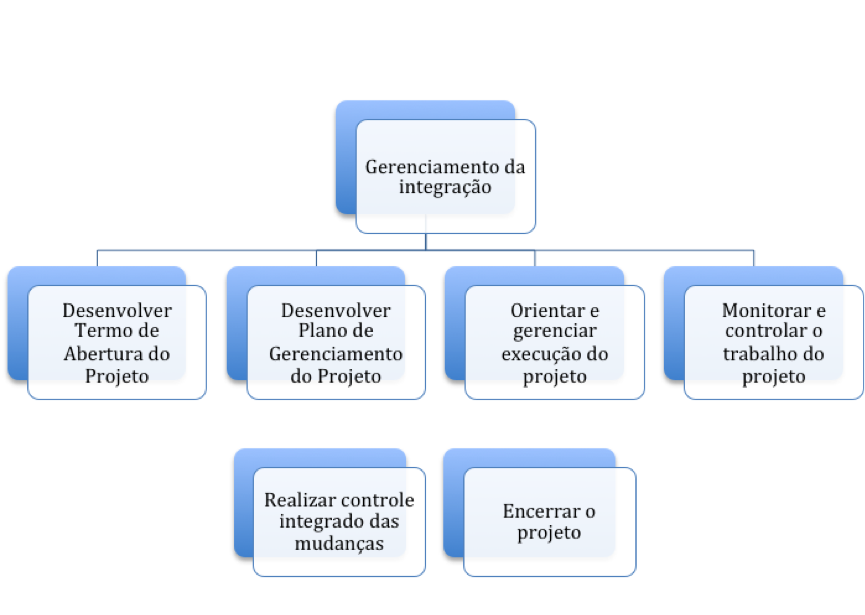
\includegraphics[scale=0.75]{Figuras/gerenciamento_integracao.png}
\caption{Processos do Gerenciamento da Integração}
\label{fig:proc:ger:integr}
\end{figure}

\section{\planproj}

O \planproj é um documento usado no auxílio da gerência do projeto no seu dia a dia. Ele é formalizado e aprovado pelos \stake e deve conter informações realistas sobre o projeto.

Ele é composto por:

\begin{itemize}

\item Plano do planejamento

\item Planos de gerenciamento de todas as áreas que serão controladas

\item Linha de base do escopo, cronograma e orçamento

\item Outros documentos e processos importantes para o gerenciamento do projeto

\end{itemize}

\subsection{Plano do planejamento}

É considerado como o pré-planejamento. Consiste em atribuir datas, responsáveis e tarefas com o objetivo de planejar o projeto e gerar os documentos e informações necessárias para a \kick. A Figura \ref{fig:plano:planejamento} mostra um exemplo de plano contendo algumas das tarefas mais importantes.

\begin{figure}[!h]
\centering
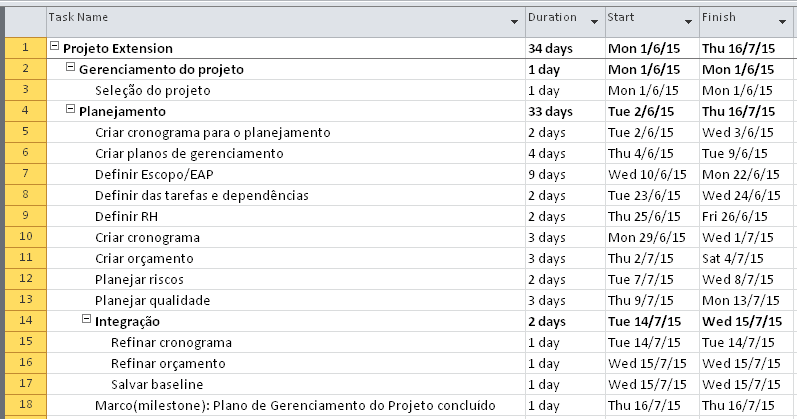
\includegraphics[scale=0.5]{Figuras/plano_planejamento.png}
\caption{Exemplo de Plano do Planejamento}
\label{fig:plano:planejamento}
\end{figure}

\subsection{\Kick}

É o evento que formaliza o início do projeto e que tem como um dos objetivos principais deixar claro os papéis e responsabilidades de todos no projeto. Por isso a participação de todos os \stake é de suma importância. Trata-se de uma ótima oportunidade de colocar frente a frente a equipe, clientes e outros \stake.

\subsection{Integracão dos planos}

Um projeto é como um organismo vivo no qual uma deficiência em uma área pode influenciar uma ou mais outras áreas. Quanto mais tarde essa deficiência for detectada e corrigida, piores serão as consequências.

Por este motivo, os planos de gerenciamento das diversas áreas do projeto não podem ser considerados totalmente independentes e devem ser construídos e mantidos de forma integrada.

Os planos de gerenciamento do projeto seguem as áreas de conhecimento que serão estudadas:

\begin{itemize}

\item \planesc
\item \plancron
\item \plancusto
\item \planqual
\item \planpess
\item \plancom
\item \planrisco
\item \planaq

\end{itemize}

Organizações que possuem escritórios de projeto (PMO) podem definir planos de gerenciamentos padronizados para que não se perca tempo com processos que se repetem em cada novo projeto. Neste caso, cabe ao \gp seguir os processos e planos definidos e o Plano do Planejamento vai incluir somente o cronograma das etapas.

\subsection{Processo Desenvolver o \planproj}

\begin{figure}[!h]
\centering
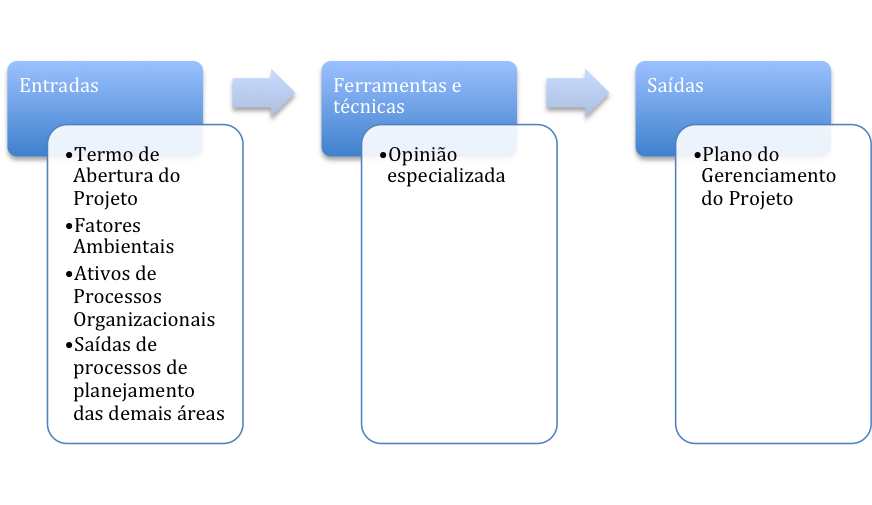
\includegraphics[scale=0.75]{Figuras/proc_integracao_1.png}
\caption{Processo Desenevolver o \planproj}
\label{fig:proc:des:planproj}
\end{figure}

\subsubsection{Entradas}

\begin{itemize}

\item \termo: principal base para início do planejamento, pois possui tudo que ja foi definido para o projeto até o momento.

\item \amb: cultura, infraestrutura, mercado, normas, etc.

\item \ativ: processos e métodos pré-definidos, informações históricas, lições aprendidas, etc.

\item Saidas de processos de planejamento das demais áreas: geram documentos e informações que devem ser integradas para a criação do \planproj. Alterações nestes planos geram alterações no \planproj.

\end{itemize}

\subsubsection{Ferramentas e técnicas}

Opinião especializada:

\begin{itemize}

\item Entender as necessidades do projeto e customizar os processos de acordo

\item Desenvolver e incluir no \planproj detalhes de nível técnico ou gerencial

\item Determinar recursos e conhecimentos necessários para execução do \planproj.

\item Identificar quais documentos necessitam de um processo formal de controle de mudanças.

\end{itemize}

\subsubsection{Saídas}

\planproj.

\subsection{Conteúdo do \planproj}

Além dos demais planos de gerenciamento, o \planproj deve definir:

\begin{itemize}

\item Controle de criação de documentos: quais documentos são necessários, quem tem a responsabilidade de criá-los e quando.

\item Planos auxiliares para gerenciamento das áreas de conhecimento.

\item Linhas de base do escopo, tempo e custo e a formalização dos processos de mudança dessas linhas de base.

\item Processo de controle de mudança:

	\begin{itemize}

	\item Pessoas autorizadas a requisitar mudanças.

	\item Processo de solicitação de mudanças.

	\item Fluxo/processo da mudança:

		\begin{itemize}

		\item Recepção
		\item Análise/avaliação
		\item Classificação
		\item Aprovação
		\item Priorização

		\end{itemize}

\end{itemize}

\end{itemize}

% !TEX root = Apostila GP.tex

\chapter{Gerenciamento do Escopo}

\section{O que é escopo}

Segundo \cite{pmbok}, escopo  é  todo  o  trabalho,  e  somente  o  trabalho  necessário  para  que  o  produto  ou 
serviço objetivo do projeto seja entregue ao seu final.

Esse é o \textbf{Escopo do projeto} que não deve ser confundido com o \textbf{Escopo do produto}, que são os atributos, funcionalidades e características que devem estar presentes no produto ou serviço criado pelo projeto, conforme podemos observar na Figura \ref{fig:escopo:proj:prod}.

\begin{figure}[!h]
\centering
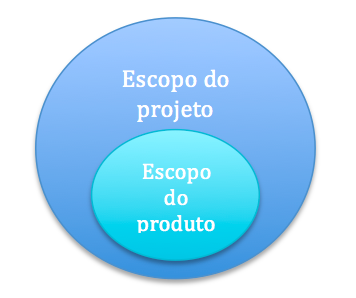
\includegraphics[scale=0.5]{Figuras/escopo_proj_prod.png}
\caption{Escopo produto X escopo projeto}
\label{fig:escopo:proj:prod}
\end{figure}

\section{Gerenciamento do Escopo}

Sãos os processos que visam garantir que o projeto inclua todo o trabalho necessários para completar com sucesso o projeto.

Para isso, deve incluir:

\begin{itemize}

\item Definir e controlar o que \textbf{faz} e o que \textbf{não faz} parte do projeto.

\item Controlar se todo o trabalho está sendo realizado.

\item Controlar o processo de mudanças do escopo.

\item Confrontar as mudanças com o \termo.

\item Evitar retrabalho ou trabalho desnecessário e seus custos

\end{itemize}

\section{Processos}

Para garantir a gerência do escopo, são necessários os seguintes processos:

\begin{itemize}

\item \textbf{Coleta de requisitos}: definir e documentar o que é necessário para se alcançar os objetivos do projeto.

\item \textbf{Definição do escopo}: descrição detalhada do projeto e do produto.

\item \textbf{Criação da Estrutura Analítica do Projeto (EAP)}: a fim de facilitar o gerenciamento das entregas e do trabalho, o escopo deve ser dividido em partes menores e estruturadas.

\item \textbf{Verificação do escopo}: formalizar a aceitação das entregas finalizadas do projeto.

\item \textbf{Controle do escopo}: monitorar e gerenciar o andamento e as mudanças na linha de base do escopo.

\end{itemize}

Os processos dentro do ciclo de vida do projeto podem ser observados na Figura \ref{fig:ciclo:vida}.

\begin{figure}[!h]
\centering
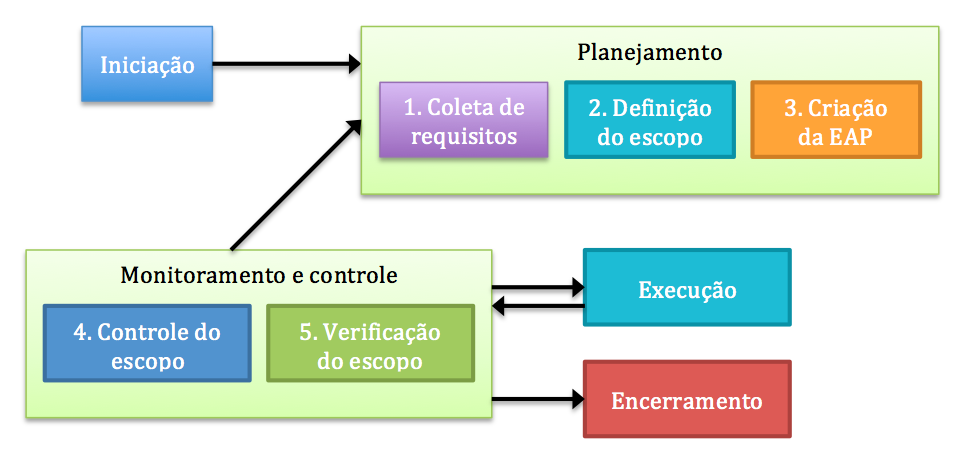
\includegraphics[scale=0.5]{Figuras/ciclo_vida.png}
\caption{Processos dentro do ciclo de vida do projeto}
\label{fig:ciclo:vida}
\end{figure}

\subsection{Inimigos do escopo}

Um escopo com problemas pode levar o projeto ao seu fim. Por isso é importante observar os dois principais inimigos do escopo:

\begin{itemize}

\item \textbf{\textit{Scope Creep}}: aumento do escopo sem nenhum controle, de maneira contínua, muitas vezes de forma lenta, que resulta em um escopo ``inchado'', ingerenciável, cujo foco foge da ideia inicial do projeto e o resultado reflete no aumento dos custos e perda de prazos.

\item \textbf{\textit{Gold Plating}}: adicionar elementos não especificados nos requisitos do projeto, geralmente partindo de equipes técnicas e de desenvolvimento sob a alegação de agregar valor mas cujo resultado é o aumento de custos, perda de qualidade e aumento desnecessário da complexidade do produto.

\end{itemize}

\subsection{Requisitos}

São condições ou capacidades que devem ser supridas pelo resultado do projeto (produto ou serviço) a fim de satisfazer um contrato ou outro documento formal.

São dividos em:

\begin{itemize}

\item \textbf{Requisitos funcionais:} o que o produto ou serviço deve \textbf{fazer}.

\item \textbf{Requisitos não-funcionais:} o que o produto ou serviço deve \textbf{ter}.

\end{itemize}

% !TEX root = Apostila GP.tex

\capitulo{Tempo}

Para gerenciramos o tempo, é preciso primeiramente termos o escopo bem definido, pois o último é base para o primeiro.

\section{Definir atividades}

A partir da EAP vamos traçar a fronteira entre o escopo e o tempo. Isso é feito através da definição das atividades.

Escopo é \textbf{o que} o projeto vai entregar. As atividades são o \textbf{como}, ou seja, de que forma o projeto vai realizar as entregas. A Tabela \ref{tab:ativ:ex} traz alguns exemplos de atividades associadas ao escopo.

\begin{table}[h!]\footnotesize
\centering
\begin{tabular}
{
 	|p{1,8cm}
	| >{\centering\arraybackslash}p{4,9cm}|
}

	\hline

	\multicolumn{2}{c}{Projeto ``Cadeira''}\\
	
	\hline
	
	Escopo&
	Atividade\\
	
	\hline

	Braço&
	\begin{itemize}
		\item Cortar madeira
		\item Lixar
		\item Colar
		\item Envernizar
	\end{itemize}\\
	
	\hline

	Assento&
	\begin{itemize}
		\item Cortar pano
		\item Cortar espuma
		\item Costurar
	\end{itemize}\\

	\hline

\end{tabular}
\caption {Exemplo de lista de atividades}
\label{tab:ativ:ex}
\end{table}

\section{Sequenciar atividades}

Sequenciar é definir a ordem e também as dependências das atividades.

\section{Estimar os recursos das atividades}

Quais os recursos materiais, humanos e tecnológicos que serão necessários para executar cada uma das atividades?

\section{Estimar as durações das atividades}

Quanto tempo será necessário para se concluir cada uma das atividades?

\section{Desenvolver o cronograma}

Um cronograma deve conter:

\begin{itemize}

\item A EAP associada à lista de atividades;

\item O sequenciamento das atividades;

\item Os recursos estimados;

\item As durações estimadas das atividades;

\item As datas reais de início e fim das atividades.

\end{itemize}

A Figura \ref{fig:ativ:ex} traz um exemplo de crongrama contendo todos os elementos citados acima.

\begin{figure}[!h]
\centering
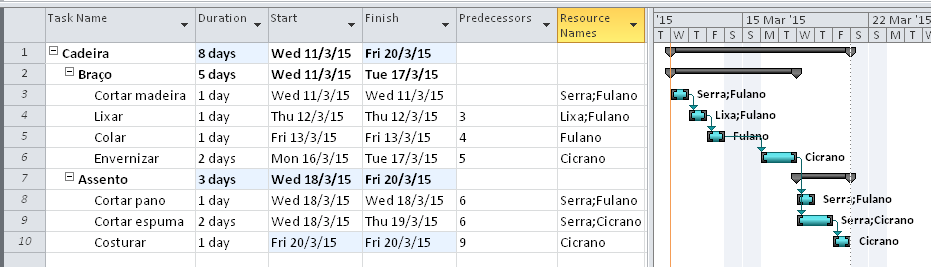
\includegraphics[scale=0.45]{Figuras/ativ_exemplo.png}
\caption{Exemplo de cronograma}
\label{fig:ativ:ex}
\end{figure}
% !TEX root = Apostila GP.tex

\capitulo{Custos}

\secao{Objetivos e características}

Abrange planejamento, estimativas, orçamentos, financiamentos, gerenciamento e controle dos custos. O principal objetivo é terminar o projeto dentro do orçamento aprovado.

O gerenciamento dos custos do projeto deve levar em consideração como as partes interessadas desejam que esse controle seja feito. Cada parte pode medir os custos de forma diferente.

Basicamente os custos do projeto são medidos pelos valores dos recursos necessários para se completar as atividades do projeto. Mas também se deve considerar os efeitos de decisões sobre custos recorrentes de utilização, manutenção e suporte do produto, serviço ou resultado do projeto. Por exemplo, limitar o número de testes de um produto pode aumentar seu custo de manutenção.

Os processos que fazem parte do gerenciamento dos custos, representados na Figura \ref{fig:proc:ger:custos}, podem ser resumidos em:

\begin{description}
	
	\item[\textbf{Planejar o gerenciamento dos custos}]: estabelecer políticas, procedimentos e documentação para planejar, gerenciar, gastar e controlar os custos do projeto.
	
	\item[\textbf{Estimar os custos}]: desenvolver uma aproximação dos recursos monetários necessários para completar as atividades do projeto.

	\item[\textbf{Definir o orçamento}]: agregar os custos estimados individuais das atividades ou pacotes de trabalho para estabelecer uma linha de base de custos autorizada.
	
	\item[\textbf{Controlar os custos}]: monitorar o progresso do projeto para atualizar os custos e gerenciar as mudanças feitas na linha de base do custo.	

\end{description}

\begin{figure}[!h]
	\centering
	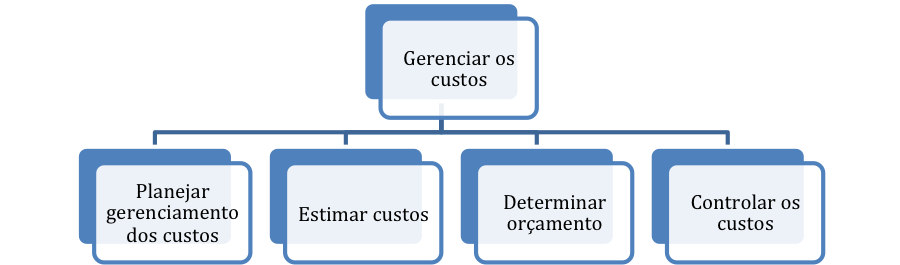
\includegraphics[scale=0.75]{Figuras/gerenciamento_custos.png}
	\caption{Processos do Gerenciamento do escopo}
	\label{fig:proc:ger:custos}
\end{figure}

\secao{Planejar gerenciamento do custo}

O plano de gerenciamento do custo estabelece políticas, procedimentos e documentação para planejar, gerenciar, gastar e controlar os custos do projeto.

O processo de planejar o gerenciamento do custo está representado na Figura \ref{fig:custos:plan:efts} e será descrito a seguir.

\begin{figure}[!h]
	\centering
	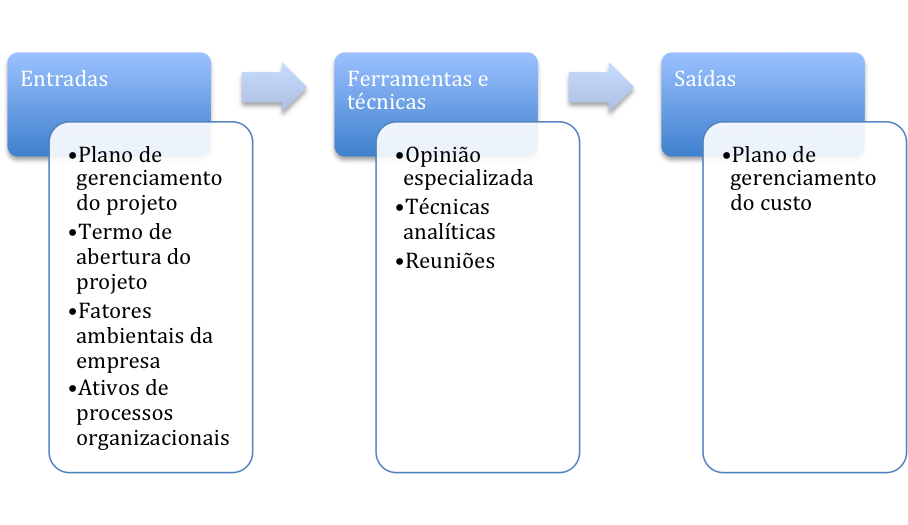
\includegraphics[scale=0.5]{Figuras/custos_efts_planejar.png}
	\caption{Planejar o gerenciamento do custo: entradas, ferramentas, técnicas e saídas}
	\label{fig:custos:plan:efts}
\end{figure}

\section{Entradas}

\begin{description}
	
	\item[Plano de gerenciamento do projeto:] contém informações importantes para se planejar o gerenciamento do custo, como a linha de base do escopo, linha de base do cronograma, entre outros.

	\item[Termo de abertura do projeto:] possui os custos em alto nível e requisitos que possam afetar o orçamento.

	\item[Fatores ambientais da empresa:] cultura, infraestrutura, condições de mercado, cotações de moedas estrangeiras, etc.

	\item[Ativos de processos organizacionais:] políticas e procedimentos internos, informações históricas, lições aprendidas, bancos de dados financeiros, etc.

\end{description}

\section{Ferramentas e técnicas}

\begin{description}

	\item[opinião especializada:] guiado por informações históricas, o especialista pode oferecer \textit{insights} valiosos sobre o ambiente e informações sobre projetos similares passados.

	\item[Técnicas analíticas:] ajudam nas decisões estratégicas sobre financiamento do projeto.
	
	\item[Reuniões:] podem participar o gerente de projetos, o patrocinador, membros selecionados da equipe, partes interessadas também selecionadas, qualquer pessoa responsável pelos custos do projeto, entre outros.
	
\end{description}

\section{Saídas}

\begin{description}
	
	\item[Plano de gerenciamento dos custos:] é um componente do \planproj e descreve como os custos serão planejados, estruturados e controlados.

\end{description}

\secao{Estimar os custos}

Processo de desenvolver uma aproximação dos recursos monetários necessários para completar as atividades do projeto. 

O processo de estimar os custos está representado na Figura \ref{fig:custos:estimar:efts} e será descrito a seguir.

\begin{figure}[!h]
	\centering
	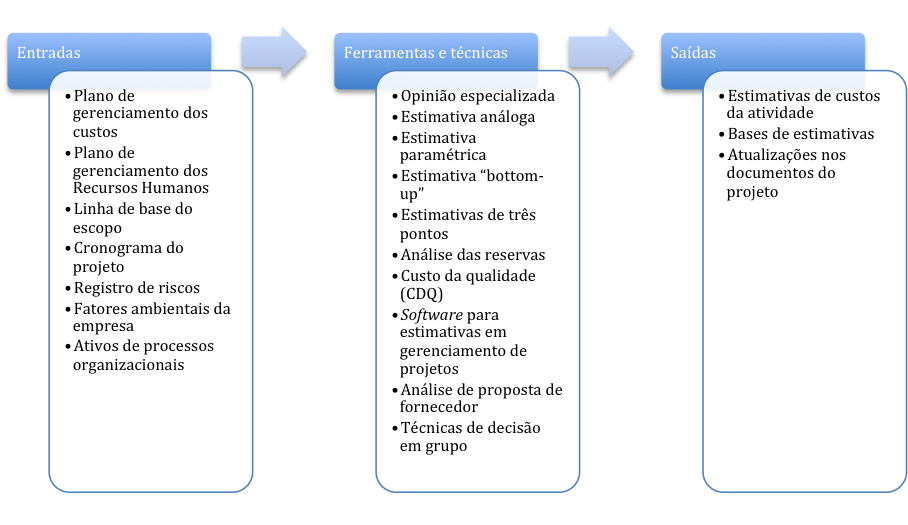
\includegraphics[scale=0.5]{Figuras/custos_efts_estimar.png}
	\caption{Estimar custos: entradas, ferramentas, técnicas e saídas}
	\label{fig:custos:estimar:efts}
\end{figure}

\section{Entradas}

\begin{description}

	\item[Plano de gerenciamento dos custos:] define comos os custos serão gerenciados e controlados.

	\item[Plano de gerenciamento dos Recursos Humanos:] oferece valores referentes aos recursos humanos que serão utilizados nas estimativas.

	\item[Linha de base do escopo:] oferece valores referentes ao produto, serviço ou resultado do projeto que serão utilizados nas estimativas.

	\item[Cronograma do projeto:] onde são encontrados a quantidade de recursos e o tempo de utilização destes recursos para estimar os custos.

	\item[Registro dos riscos:] o custo de resposta aos riscos deve ser considerado.
	
	\item[Fatores ambientais da empresa:] condições de mercado, informações comerciais publicadas, etc.
	
	\item[Ativos de processos organizacionais:] políticas de estimativa de custos, modelos de estimativas de custos, informações históricas, lições aprendidas, etc.
	
\end{description}

\section{Ferramentas e técnicas}

\begin{description}
	
	\item[Opinião especializada:] guiado por informações históricas, o especialista pode oferecer \textit{insights} valiosos sobre o ambiente e informações sobre projetos similares passados.
	
	\item[Estimativa análoga:] utiliza valores de projetos similares passados como parâmetro para estimativa dos custos.
	
	\item[Estimativa paramétrica:] utiliza relacionamento estatístico entre informações históricas relevantes e outras variáveis (por exemplo, $m^2$ construído) para calcular a estimativa de custos.
	
	\item[Estimativa \textit{bottom-up}:] custos de pacotes de trabalho individuais ou atividades são estimados e posteriormente resumidos nos níveis mais altos.
	
	\item[Estimativa de três pontos:] utiliza três estimativas:
	
		\begin{itemize}
			\item Mais provável (cM) - realista;
			\item Otimista (cO) - cenário ideal;
			\item Pessimista (cP) - pior cenário.		
		\end{itemize}
		
	As duas fórmulas mais comuns para estimativa de três pontos são:
	
		\begin{eqnarray*}
			\text{\textbf{Distribuição triangular}}&:&cE=\frac{cO+cM+cP}{3}\\	
			&&\\	
			\text{\textbf{Distribuição beta}}&:&cE=\frac{cO+4 \times cM+cP}{6}
		\end{eqnarray*}
		
	\item[Análise de reserva:] a estimativa pode incluir reservas de contingência para resposta aos riscos, cobertura de fatos desconhecidos e pode ser destinada a uma atividade específica ou para todo o projeto. Pode ser um percentual do custo estimado total, um valor fixo ou um valor determinado através de análises quantitativas.
	
	\item[Custo da Qualidade (CDQ):] podem ser utilizado para compor a estimativa.
	
	\item[\textit{Softwares} para estimativas em gerenciamento de projetos:] aplicativos, planilhas, simuladores, ferramentas estatísticas, etc.
	
	\item[Análise de proposta de fornecedor:] as estimativas podem ser feitas através da análise de propostas de fornecedores qualificados.
	
	\item[Técnicas de tomada de decisão em grupo:] auxiliam quando múltiplas alternativas forem apresentadas.
	
		
\end{description}

\section{Saídas}

\begin{description}
	
	\item[Estimativas de custos da atividade:] avaliações quantitativas dos prováveis custos necessários para executar o trabalho do projeto.
	
	\item[Bases de estimativas:] a quantia e tipo de detalhes adicionais que suportam a estimativa dos custos variam por área de aplicação. Independentemente do nível de detalhe, a documentação de suporte deve fornecer um entendimento claro e completo a respeito de como a estimativa de custos foi derivada.

	\item[Atualizações nos documentos do projeto:] registro dos riscos, entre outros.

\end{description}

\secao{Determinar o orçamento}

Processo de agregação dos custos estimados de atividades individuais ou pacotes de trabalho para estabelecer uma linha de base dos custos autorizada. 

O processo de determinar o orçamento está representado na Figura \ref{fig:custos:orcamento:efts} e será descrito a seguir.

\begin{figure}[!h]
	\centering
	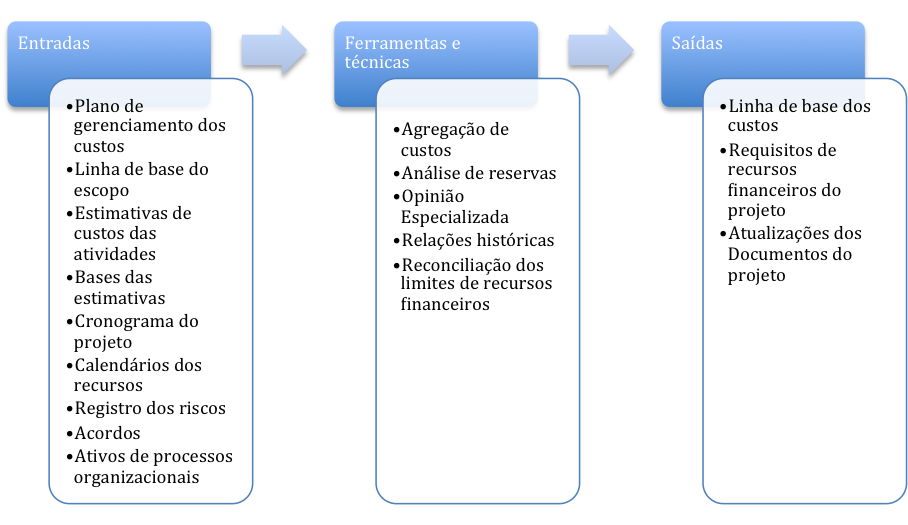
\includegraphics[scale=0.5]{Figuras/custos_efts_orcamento.png}
	\caption{Determinar o orçamento: entradas, ferramentas, técnicas e saídas}
	\label{fig:custos:orcamento:efts}
\end{figure}

\section{Entradas}

\begin{description}

	
	\item[Plano de gerenciamento dos custos:] descreve como os custos serão gerenciados e controlados.

	\item[Linha de base do escopo:] oferece informações sobre limitações, relacionamento entre pacotes de trabalho, etc.
	
	\item[Estimativas de custos das atividades:] serão agregadas para gerar as estimativas dos pacotes de trabalho.
	
	\item[Bases das estimativas:] informações adicionais sobre as estimativas.
	
	\item[Cronograma do projeto:] contém informações que podem ser usadas para agregar custos nos períodos do calendário em que os custos são planejados a incorrerem.
	
	\item[Calendários dos recursos:] contém informações que podem ser usadas para indicar os custos dos recursos durante o projeto.
	
	\item[Registro dos riscos:] deve ser revisado para considerar como os custos de resposta aos riscos serão agregados.
	
	\item[Acordos:] produtos, serviços ou outros que serão comprados durante o projeto deverão ser considerados.
	
	\item[Ativos de processos organizacionais:] políticas, procedimentos e diretrizes existentes, formais ou informais, relacionadas ao orçamento de custos, ferramentas para orçamento de custos, métodos de elaboração de relatórios, etc.
	
\end{description}

\section{Ferramentas e técnicas}

\begin{description}

	\item[Agregação de custos:] pacotes de trabalho $\rightarrow$ níveis superiores $\rightarrow$ projeto todo.
	
	\item[Análise de reservas:] reservas de contingência e reservas gerenciais.
	
	\item[Opinião Especializada:] pessoas, grupos ou empresas que possam auxiliar na determinação do orçamento.
	
	\item[Relações históricas:] quaisquer relações históricas que resultam em estimativas paramétricas ou análogas envolvem o uso de características de projetos (parâmetros) para desenvolver modelos matemáticos para prever o custo total do projeto.
	
	\item[Reconciliação dos limites de recursos financeiros:] a utilização de fundos deve ser reconciliada com quaisquer limites de recursos de fundos alocados ao projeto.
		
\end{description}

\section{Saídas}

\begin{description}
	
	\item[Linha de base dos custos:] é a versão aprovada do orçamento do projeto, sincronizado com o tempo, excluindo qualquer reserva gerencial, que só pode ser modificada através de um controle formal de mudanças e é utilizada como base de comparação com os resultados reais.
	
	\item[Requisitos de recursos financeiros do projeto:] gastos projetados mais responsabilidades antecipadas.
	
	\item[Atualizações dos Documentos do projeto:] registro dos riscos, estimativa de custos, cronograma do projeto, etc.

	
\end{description}

\secao{Controlar os custos}

Processo de monitoramento do progresso do projeto para atualização do seu orçamento e gerenciamento das mudanças feitas na linha de base dos custos.

O processo de controlar os custos está representado na Figura \ref{fig:custos:controlar:efts} e será descrito a seguir.

\begin{figure}[!h]
	\centering
	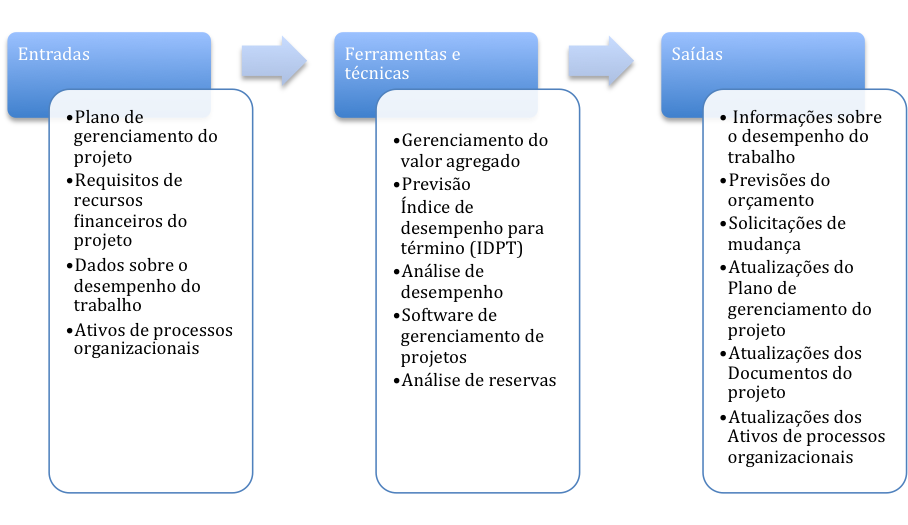
\includegraphics[scale=0.5]{Figuras/custos_efts_controlar.png}
	\caption{Controlar os custos: entradas, ferramentas, técnicas e saídas}
	\label{fig:custos:controlar:efts}
\end{figure}

\section{Entradas}

\begin{description}
	
	\item[Plano de gerenciamento do projeto:] utiliza a linha de base do desempenho de custos e o plano de gerenciamento dos custos.
	
	\item[Requisitos de recursos financeiros do projeto:] despesas do projeto e obrigações antecipadas.
	
	\item[Dados sobre o desempenho do trabalho:] custos já autorizados e incorridos.
	
	\item[Ativos de processos organizacionais:] políticas, procedimentos e diretrizes existentes, formais ou informais, relacionadas ao controle de custos, ferramentas de controle de custos e métodos de monitoramento e relato de informações a serem utilizados.
	
\end{description}

\section{Ferramentas e técnicas}

\begin{description}
	
	\item[Gerenciamento do valor agregado:] integra as medidas de escopo, custos e cronograma para auxiliar a equipe de gerenciamento a avaliar e medir o desempenho e progresso do projeto.
	
	\item[Previsão:] envolve a execução de estimativas ou prognósticos de condições e eventos no futuro do projeto com base nas informações e conhecimento disponíveis no momento da previsão.
	
	\item[Índice de desempenho para término (IDPT):] projeção calculada do desempenho de custos que deve ser atingido no trabalho restante para alcançar um objetivo de gerenciamento especificado.
	
	\item[Análise de desempenho:] compara o desempenho de custos através do tempo, atividades do cronograma ou pacotes de trabalho acima e abaixo do orçamento e recursos financeiros estimados necessários para terminar o trabalho em progresso.
	
	\item[Software de gerenciamento de projetos:] usado para monitorar os custos, mostrar tendências e prever resultados.
	
	\item[Análise de reservas:] monitorar o status das reservas de contingência e gerencial e determinar se são suficientes ou se será necessário requisitar reservas adicionais.
	
\end{description}

\section{Saídas}

\begin{description}
	
	\item[Informações sobre o desempenho do trabalho:] documentação e comunicação dos índices dos custos.
	
	\item[Previsões do orçamento:] informações sobre o orçamento são documentadas e comunicadas às partes interessadas.
	
	\item[Solicitações de mudança:] a análise do desempenho do projeto pode resultar numa solicitação de mudança da linha de base do desempenho de custos ou de outros componentes do plano de gerenciamento do projeto.
	
	\item[Atualizações do Plano de gerenciamento do projeto:] linha de base do desempenho de custos, plano de gerenciamento dos custos, etc.
	
	\item[Atualizações dos Documentos do projeto:] estimativa de custos, bases de estimativas, etc.
	
	\item[Atualizações dos Ativos de processos organizacionais:] causas de variações, ações corretivas escolhidas e suas razões, bancos de dados financeiros, lições aprendidas a partir do controle de custos, etc.
	
\end{description}
% !TEX root = Apostila GP.tex

\capitulo{Qualidade}

\secao{Objetivos e características}

O gerenciamento da qualidade do projeto inclui processos e atividades da organização executora que determinam políticas, objetivos e responsabilidades referentes a qualidade, a fim de que o projeto satisfaça as necessidades para o qual foi empreendido. O gerenciamento da qualidade do projeto utiliza políticas e procedimentos para implementar, dentro do contexto do projeto, o sistema de gestão da qualidade da organização e suporta atividades de melhoria contínua de processos. O gerenciamento da qualidade do projeto trabalha para garantir que os requisitos do projeto, incluindo os requisitos do produto, sejam alcançados e validados.

Os processos que fazem parte do gerenciamento da qualidade, representados na Figura \ref{fig:proc:ger:qualidade}, podem ser resumidos em:

\begin{description}
	
	\item[\textbf{Planejar o Gerenciamento da Qualidade}]: identificar os requisitos e/ou padrões para o projeto e suas entregas e documentar como o projeto irá atendê-los.
	
	\item[\textbf{Realizar a garantia da qualidade}]: auditar os requisitos de qualidade e os resultados das medidas do controle de qualidade para garantir que os padrões apropriados de qualidade e as definições operacionais estejam sendo utilizadas.
	
	\item[\textbf{Controlar a qualidade}]: monitorar e registrar os resultados de execução das atividades de qualidade para avaliar o desempenho e recomendar as mudanças necessárias.

\end{description}

\begin{figure}[!h]
	\centering
	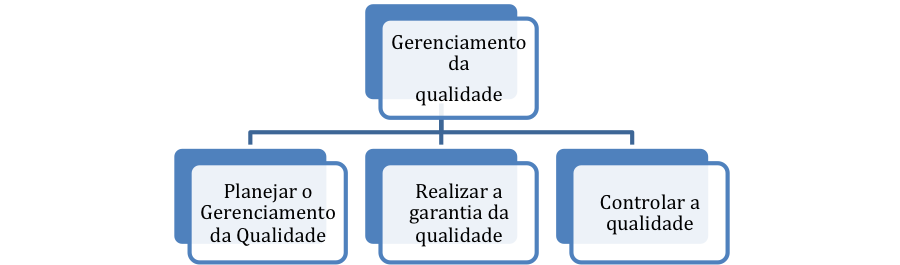
\includegraphics[scale=0.75]{Figuras/gerenciamento_qualidade.png}
	\caption{Processos do gerenciamento da qualidade}
	\label{fig:proc:ger:qualidade}
\end{figure}

\secao{Planejar o Gerenciamento da Qualidade}

O plano de gerenciamento da qualidade é o processo de identificar os requisitos e/ou padrões para o projeto e suas entregas e documentar como o projeto irá atendê-los.

O processo de planejar o gerenciamento da qualidade está representado na Figura \ref{fig:qualidade:plan:efts} e será descrito a seguir.

\begin{figure}[!h]
	\centering
	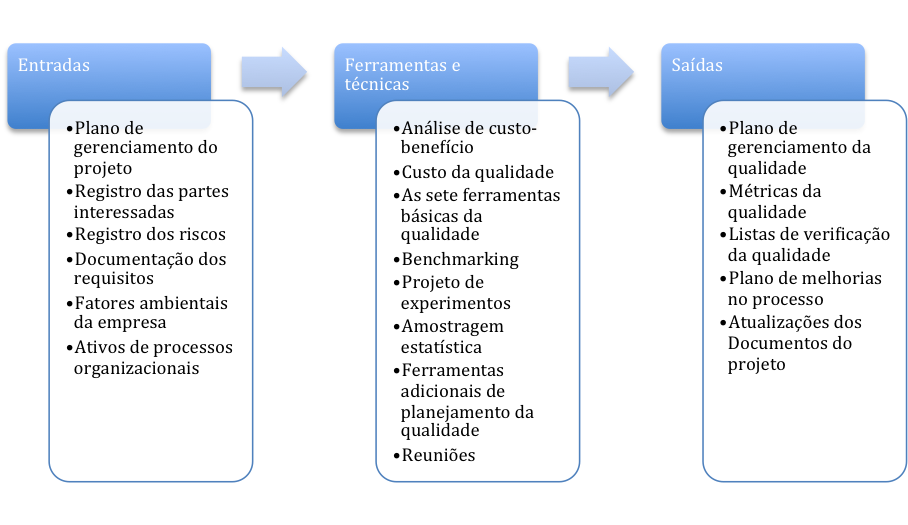
\includegraphics[scale=0.5]{Figuras/qualidade_efts_planejar.png}
	\caption{Planejar o gerenciamento da qualidade: entradas, ferramentas, técnicas e saídas}
	\label{fig:qualidade:plan:efts}
\end{figure}

\section{Entradas}

\begin{description}
	
	\item[Plano de gerenciamento do projeto:] inclui informações utilizadas no desenvolvimento do plano de gerenciamento da qualidade (linha de base do escopo, do cronograma e do custo, entre outros documentos).
	
	\item[Registro das partes interessadas:] auxilia na identificação de quem possua um interesse particular ou tenha um impacto na qualidade.
	
	\item[Registro dos riscos:] contém informações sobre ameaças e oportunidades que possam impactar nos requisitos de qualidade.
	
	\item[Documentação dos requisitos:] capturam os requisitos que o projeto deve atender pertinentes às expectativas das partes interessadas.
	
	\item[Fatores ambientais da empresa:] regulamentações de agências governamentais, regras, padrões e diretrizes específicas para uma área de aplicação, condições de operação ou de trabalho do projeto ou das entregas que possam afetar a qualidade do projeto, percepções culturais que possam influenciar as expectativas sobre a qualidade, etc.
	
	\item[Ativos de processos organizacionais:] políticas, procedimentos e diretrizes organizacionais, bancos de dados históricos, lições aprendidas, etc.
	
\end{description}

\section{Ferramentas e técnicas}

\begin{description}

	\item[Análise de custo-benefício:] compara o custo de cada atividade da qualidade com seu benefício esperado.
	
	\item[Custo da qualidade:] são os custos usados para prevenir a não conformidade, ou seja, o dinheiro gasto durante o projeto para evitar falhas. Entre eles:
	
	\begin{itemize}
		
		\item Custos de conformidade
					
		\begin{itemize}

			\item Prevenção de custos (Fabricar um produto de qualidade)
			
			\begin{itemize}
				
				\item Treinamento;
				
				\item Documentar processos;
				
				\item Equipamento;
				
				\item Tempo para executar do modo correto.
				
			\end{itemize}
			
			\item Custos de avaliação (Avaliar a qualidade)
			
			\begin{itemize}
				
				\item Testes;
				
				\item Perda de teste destrutivo;
				
				\item Inspeções.
				
			\end{itemize}
			
		\end{itemize}
	
		\item Custos de não conformidade
		
		\begin{itemize}
		
			\item Custos de falhas internas (Falhas encontradas pelo projeto)
			
			\begin{itemize}
				
				\item Retrabalho;
				
				\item Descarte.
				
			\end{itemize}
			
			\item Custos de falhas externas (Falhas encontradas pelo cliente)	
			
			\begin{itemize}
				
				\item Responsabilidades;
				
				\item Trabalho de garantia;
				
				\item Perda de negócios.

			\end{itemize}
						
		\end{itemize}
	
	\end{itemize}

	\item[As sete ferramentas básicas da qualidade:] também conhecidas como \textit{7QC Tools}.
	
		\begin{itemize}
			\item Diagrama de causa-efeito
			\item Fluxograma
			\item Folha de verificação
			\item Histograma
			\item Diagrama de Pareto
			\item Gráfico de controle
			\item Diagrama de dispersão			
		\end{itemize}
	
	\item[Benchmarking:] é o processo de comparar os métodos de trabalho em relação às melhores práticas e resultados com o propósito de identificar mudanças que levem a resultados de melhor qualidade.
	
	\item[Projeto de experimentos:] método estatístico que ajuda a identificar quais fatores podem influenciar variáveis específicas de um produto ou processo em desenvolvimento.
	
	\item[Amostragem estatística:] tem como objetivo fazer generalizações sobre uma população com base nos dados de uma amostra.
	
	\item[Ferramentas adicionais de planejamento da qualidade:] alguns exemplos:
	
	\begin{itemize}
		
			\item Brainstorming;
			
			\item Técnica de grupo nominal;
			
			\item Diagramas Matriciais;
			
			\item Matriz de priorização.
			
	\end{itemize}
		
	\item[Reuniões:] utilizadas para auxiliar no desenvolvimento do plano de gerenciamento da qualidade.
		
\end{description}

\section{Saídas}

\begin{description}
	
	\item[Plano de gerenciamento da qualidade:] descreve como as políticas de qualidade da organização serão implementadas.
	
	\item[Plano de melhoria de processos:] detalha os passos para analisar os processos de gerenciamento de projeto e desenvolvimento de produto para identificar atividades que possam aumentar seus valores.
	
	\item[Métricas da qualidade:] descreve um atributo do projeto ou do produto e como o processo de controle de qualidade irá mensurá-lo.
	
	\item[Listas de verificação da qualidade:] utilizada para verificar se um conjunto de passos requeridos foram executados.
	
	\item[Atualizações dos Documentos do projeto:] registro de partes interessadas, matriz de atribuição de responsabilidades, EAP e dicionário da EAP, etc.
		
\end{description}

\secao{Realizar a garantia da qualidade}

Processo de auditar os requisitos de qualidade e os resultados das medidas do controle de qualidade para garantir que os padrões apropriados de qualidade e as definições operacionais estejam sendo utilizadas.

O processo de realizar a garantia da qualidade está representado na Figura \ref{fig:qualidade:gar:efts} e será descrito a seguir.

\begin{figure}[!h]
	\centering
	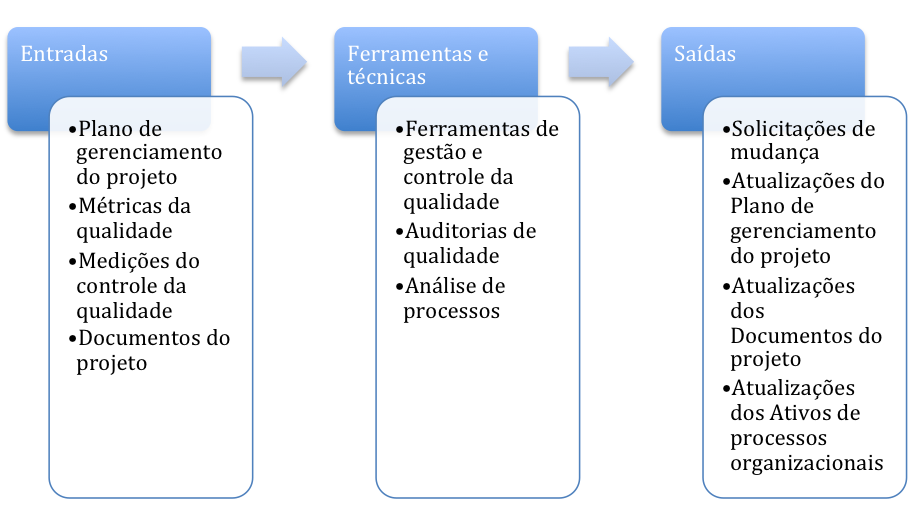
\includegraphics[scale=0.5]{Figuras/qualidade_efts_realizar.png}
	\caption{Realizar a garantia da qualidade: entradas, ferramentas, técnicas e saídas}
	\label{fig:qualidade:gar:efts}
\end{figure}

\section{Entradas}

\begin{description}

	\item[Plano de gerenciamento da qualidade:] descreve a abordagem da garantia da qualidade e da melhoria contínua de processos do projeto.
	
	\item[Plano de melhoria dos processos:] as atividades de garantia da qualidade do projeto devem ser consistentes e apoiar os planos de melhoria de processos da organização.
	
	\item[Métricas da qualidade:] indicam os atributos que devem ser mensurados e as variações toleráveis.
	
	\item[Medições do controle da qualidade:] resultados das atividades de controle da qualidade.
	
	\item[Documentos do projeto:] documentos que possam influenciar no trabalho da garantia da qualidade.
		
\end{description}

\section{Ferramentas e técnicas}

\begin{description}
	
	\item[Ferramentas de gestão e controle da qualidade:] alguns exemplos:
	
	\begin{itemize}
		
		\item Diagrama de afinidades;
		
		\item Gráfico de programa de decisão de processo (PDPC);
		
		\item Gráfico de inter relacionamento;
		
		\item Diagramas de árvore;
		
		\item Matrizes de priorização;
		
		\item Diagramas de rede;
		
		\item Diagramas de matriz.
		
	\end{itemize}
	
	\item[Auditorias de qualidade:] processo estruturado e independente que determina se as atividades do projeto estão em conformidade com as políticas, processos e procedimentos da organização e do projeto.
	
	\item[Análise de processos:] segue os passos delineados no plano de melhoria de processos para identificar o que precisa ser melhorado.
		
\end{description}

\section{Saídas}

\begin{description}
	\item[Solicitações de mudança:] podem ser geradas para avaliação das melhorias recomendadas.
	
	\item[Atualizações do Plano de gerenciamento do projeto:] planos de gerenciamento da qualidade, escopo, tempo e custo, entre outros.
	
	\item[Atualizações dos Documentos do projeto:] relatórios de auditoria da qualidade, planos de treinamento, etc.
	
	\item[Atualizações dos Ativos de processos organizacionais:] padrões de qualidade, sistemas de gerenciamento da qualidade, etc.
	
\end{description}

\secao{Controlar a qualidade}

Processo de monitorar e registrar os resultados de execução das atividades de qualidade para avaliar o desempenho e recomendar as mudanças necessárias.

O processo de controlar a qualidade está representado na Figura \ref{fig:qualidade:controlar:efts} e será descrito a seguir.

\begin{figure}[!h]
	\centering
	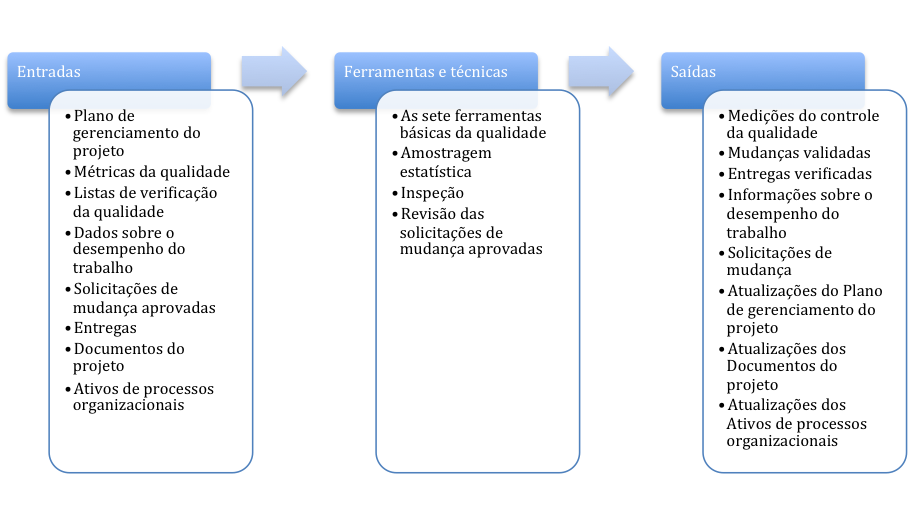
\includegraphics[scale=0.5]{Figuras/qualidade_efts_controlar.png}
	\caption{Controlar a qualidade: entradas, ferramentas, técnicas e saídas}
	\label{fig:qualidade:controlar:efts}
\end{figure}

\section{Entradas}

\begin{description}

	\item[Plano de gerenciamento do projeto:] utiliza o plano de gerenciamento da qualidade que descreve como será feito o controle da qualidade.
	
	\item[Métricas da qualidade:] descrição dos atributos e formas de mensurá-los.
	
	\item[Listas de verificação da qualidade:] lista estruturada que auxilia na verificação do trabalho do projeto e suas entregas.
	
	\item[Dados sobre o desempenho do trabalho:] permite confrontar o que foi planejado com os dados reais de trabalho.
	
	\item[Solicitações de mudança aprovadas:] podem incluir reparo de defeitos, métodos de trabalho revisados e cronograma revisado.
	
	\item[Entregas:] produto, resultado ou capacidade única e verificável do projeto que resulta em uma entrega validada requerida pelo projeto.
	
	\item[Documentos do projeto:] acordos, relatórios de auditoria da qualidade, planos de treinamento, etc.
	
	\item[Ativos de processos organizacionais:] políticas e padrões de qualidade da organização, diretrizes padrões de trabalho, etc.
	
\end{description}

\section{Ferramentas e técnicas}

\begin{description}
	
	\item[As sete ferramentas básicas da qualidade:] também conhecidas como \textit{7QC Tools}.
	
	\begin{itemize}
		\item Diagrama de causa-efeito
		\item Fluxograma
		\item Folha de verificação
		\item Histograma
		\item Diagrama de Pareto
		\item Gráfico de controle
		\item Diagrama de dispersão			
	\end{itemize}
	
	\item[Amostragem estatística:] tem como objetivo fazer generalizações sobre uma população com base nos dados de uma amostra.
	
	\item[Inspeção:] examinação de um produto de trabalho para determinar se está em conformidade com os padrões documentados.
	
	\item[Revisão das solicitações de mudança aprovadas:] todas as solicitações de mudança aprovadas devem ser revisadas para verificar se elas foram implementadas da forma como foram aprovadas.
	
\end{description}

\section{Saídas}

\begin{description}
	
	\item[Medições do controle da qualidade:] resultados documentados das atividades de controle da qualidade.
	
	\item[Mudanças validadas:] todos os itens reparados são inspecionados e serão aceitados ou rejeitados.
	
	\item[Entregas verificadas:] o objetivo do controle da garantia do projeto é determinar que as entregas sejam realizadas de forma correta.
	
	\item[Informações sobre o desempenho do trabalho:] dados coletados de vários processos de controle, analisados em contexto e integrados baseado em relacionamentos entre áreas.
	
	\item[Solicitações de mudança:] devem ser geradas para ações corretivas ou preventivas recomendadas.
	
	\item[Atualizações do Plano de gerenciamento do projeto:] plano de gerenciamento da qualidade, plano de melhoria de processos, etc.
	
	\item[Atualizações dos Documentos do projeto:] padrões de qualidade, acordos, relatórios de auditoria da qualidade, planos de treinamento, etc.
	
	\item[Atualizações dos Ativos de processos organizacionais:] lições aprendidas, etc.
	
\end{description}
% !TEX root = Apostila GP.tex

\capitulo{Recursos Humanos}

\secao{Objetivos e características}

O gerenciamento dos recursos humanos do projeto inclui os processos para organizar, gerenciar e liderar a equipe do projeto, que são as pessoas com papéis e responsabilidades atribuídos para completar o projeto.

Os processos que fazem parte do gerenciamento dos recursos humanos, representados na Figura \ref{fig:proc:ger:rh}, podem ser resumidos em:

\begin{description}

	\item[Planejar o gerenciamento dos recursos humanos:] identificar e documentar os papéis, responsabilidades e habilidades requeridas, reportar relacionamentos e criar um plano de gerenciamento da equipe.
	
	\item[Mobilizar a equipe do projeto:] confirmar a disponibilidade dos recursos humanos e obter a equipe necessária para completar as atividades do projeto.
	
	\item[Desenvolver a equipe do projeto:] melhorar as competências, interação dos membros da equipe e ambiente geral da equipe para aprimorar o desempenho do projeto.
	
	\item[Gerenciar a equipe do projeto:] acompanhar o desempenho da equipe, fornecer feedback, resolver problemas e gerenciar mudanças para otimizar o desempenho do projeto.

\end{description}

\begin{figure}[!h]
	\centering
	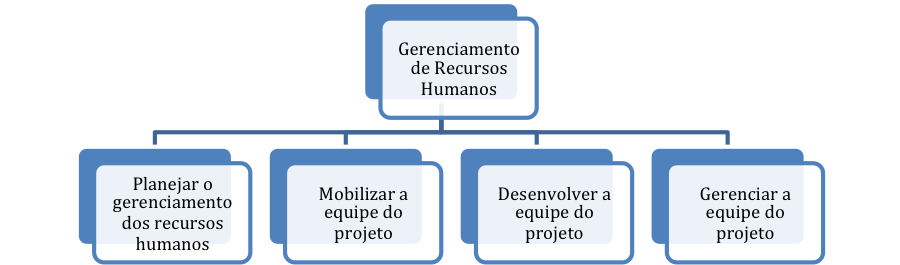
\includegraphics[scale=0.75]{Figuras/gerenciamento_rh.png}
	\caption{Processos do Gerenciamento dos recursos humanos}
	\label{fig:proc:ger:rh}
\end{figure}

\secao{Planejar o gerenciamento dos recursos humanos}

Planejar o gerenciamento dos recursos humanos é o processo de identificar e documentar os papéis, responsabilidades e habilidades requeridas, reportar relacionamentos e criar um plano de gerenciamento da equipe.

O processo de planejar o gerenciamento dos recursos humanos está representado na Figura \ref{fig:rh:plan:efts} e será descrito a seguir.

\begin{figure}[!h]
	\centering
	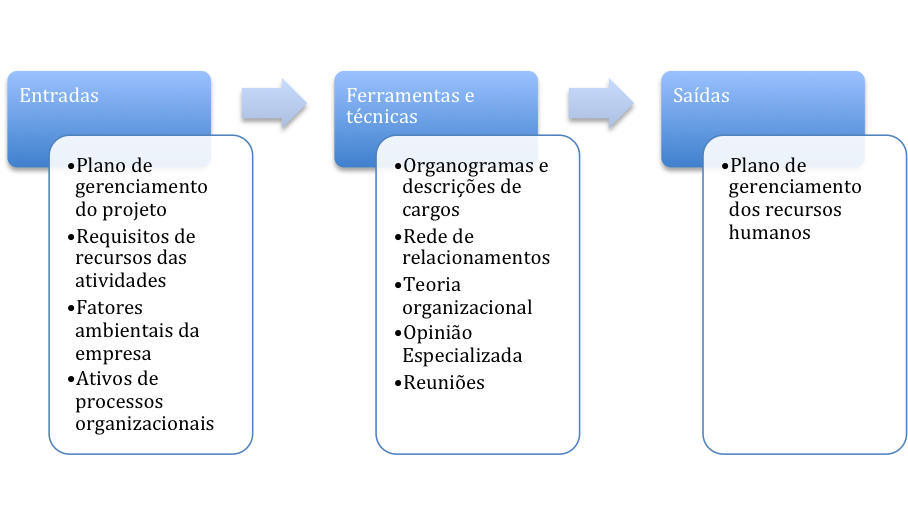
\includegraphics[scale=0.5]{Figuras/rh_efts_planejar.png}
	\caption{Planejar o gerenciamento dos recursos humanos: entradas, ferramentas, técnicas e saídas}
	\label{fig:rh:plan:efts}
\end{figure}

\section{Entradas}

\begin{description}
	
	\item[Plano de gerenciamento do projeto:] ciclo de vida e processos que serão aplicados em cada fase, como o trabalho será executado para alcançar os objetivos do projeto, plano de gerenciamento de mudanças que documenta como as mudanças serão monitoradas e controladas, plano de gerenciamento de configuração, como a integridade das linhas de base do projeto serão mantidas, necessidades e métodos de comunicação com as partes interessadas, etc.
	
	\item[Requisitos de recursos das atividades:] utilizado para determinar as necessidades de recursos humanos para o projeto.
	
	\item[Fatores ambientais da empresa:] cultura e estrutura organizacional, recursos humanos existentes, dispersão geográfica dos membros da equipe, políticas de administração de pessoal, condições de mercado, etc.
	
	\item[Ativos de processos organizacionais:] processos padronizados, políticas e descrições de papéis, modelos de organogramas e descrições de papéis, lições aprendidas sobre estruturas organizacionais que funcionaram em projetos anteriores, procedimentos de escalonamento para lidar com problemas dentro da equipe e dentro da organização, etc.
	

\end{description}

\section{Ferramentas e técnicas}

\begin{description}

	\item[Organogramas e descrições de cargos:] garantir que cada pacote de trabalho tenha um dono único e que todos os membros da equipe tenham uma compreensão clara de seus papéis e responsabilidades.
	
	\item[Rede de relacionamentos:] interações formais e informais com outras pessoas em uma organização, indústria ou ambiente profissional.
	
	\item[Teoria organizacional:] oferece informação a respeito da forma como as pessoas, equipes e unidades organizacionais se comportam.
	
	\item[Opinião Especializada:] listar requisitos preliminares para as habilidades necessárias, avaliar os papéis necessários para o projeto baseado em descrições padronizadas de papéis dentro da organização, determinar o nível de esforço preliminar e número de recursos necessários para alcançar os objetivos do projeto, determinar as subordinações necessárias baseado na cultura organzacional, oferecer orientações sobre o tempo necessário para formar a equipe, identificar riscos associados com a aquisição, retenção e desmobilização da equipe, identificar e recomendar programas para manter conformidade com contratos governamentais e sindicais, etc.
	
	\item[Reuniões:] podem ser necessárias durante o planejamento do gerenciamento dos recursos humanos.
	

\end{description}

\section{Saídas}

\begin{description}
	
	\item[Plano de gerenciamento dos recursos humanos:] plano contendo papéis e responsabilidades, organograma do projeto, plano de gerenciamento da equipe, etc.	
	
\end{description}

\secao{Mobilizar a equipe do projeto}

Processo de confirmar a disponibilidade dos recursos humanos e obter a equipe necessária para completar as atividades do projeto.

O processo de mobilizar a equipe do projeto está representado na Figura \ref{fig:rh:mob:efts} e será descrito a seguir.

\begin{figure}[!h]
	\centering
	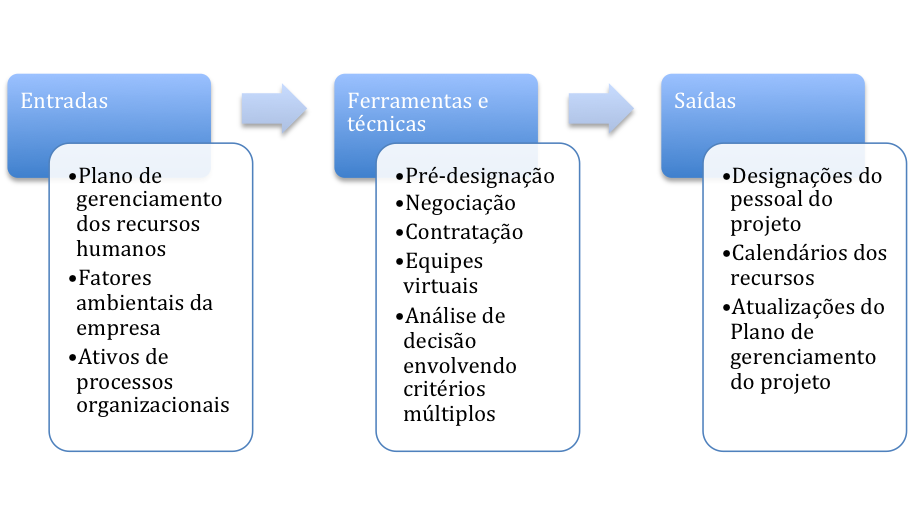
\includegraphics[scale=0.5]{Figuras/rh_efts_mobilizar.png}
	\caption{Mobilizar a equipe do projeto: entradas, ferramentas, técnicas e saídas}
	\label{fig:rh:mob:efts}
\end{figure}

\section{Entradas}

\begin{description}

	\item[Plano de gerenciamento dos recursos humanos:] oferece orientações sobre como os recursos humanos são identificados, compostos, gerenciados e eventualmente desmobilizados.
	
	\item[Fatores ambientais da empresa:] informações existentes sobre recursos humanos (disponibilidade, níveis de competência, experiência anterior, interesse em trabalhar no projeto e custos), políticas de administração de pessoal, estrutura organizacional, localização, etc.
	
	\item[Ativos de processos organizacionais:] políticas padronizadas da organização, processos, procedimentos, etc.
	
\end{description}

\section{Ferramentas e técnicas}

\begin{description}
	
	\item[Pré-designação:] ocorre quando os membros da equipe são selecionados com antecedência.
	
	\item[Negociação:] a negociação de atribuição de pessoal é necessária em diversos projetos.
	
	\item[Contratação:] quando a organização não consegue fornecer todo o pessoal necessário.
	
	\item[Equipes virtuais:] grupos de pessoas com objetivos compartilhados que cumprem seus papéis com pouco ou nenhum contato físico.
	
	\item[Análise de decisão envolvendo critérios múltiplos:] utilizados para dar notas ou pontuar potenciais membros da equipe e auxiliar na sua seleção.
	
\end{description}

\section{Saídas}

\begin{description}

	\item[Designações do pessoal do projeto:] a composição do projeto acontece quando as pessoas apropriadas forem designadas à equipe.
	
	\item[Calendários dos recursos:] documenta os períodos de tempo em que cada membro da equipe do projeto está disponível para o trabalho.
	
	\item[Atualizações do Plano de gerenciamento do projeto:] principalmente no plano de gerenciamento dos recursos humanos.
	
\end{description}

\secao{Desenvolver a equipe do projeto}

Processo de melhorar as competências, interação dos membros da equipe e ambiente geral da equipe para aprimorar o desempenho do projeto.

O processo de desenvolver a equipe do projeto está representado na Figura \ref{fig:rh:desenv:efts} e será descrito a seguir.

\begin{figure}[!h]
	\centering
	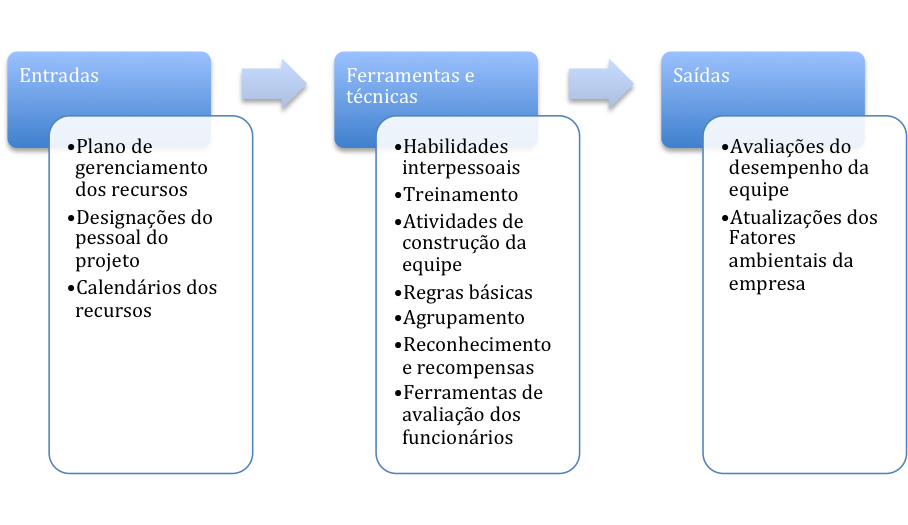
\includegraphics[scale=0.5]{Figuras/rh_efts_desenvolver.png}
	\caption{Desenvolver a equipe do projeto: entradas, ferramentas, técnicas e saídas}
	\label{fig:rh:desenv:efts}
\end{figure}

\section{Entradas}

\begin{description}

	\item[Plano de gerenciamento dos recursos:] define estratégias de treinamento e planos para desenvolvimento da equipe do projeto.
	
	\item[Designações do pessoal do projeto:] identifica as pessoas que estão na equipe.
	
	\item[Calendários dos recursos:] identifica períodos em que os membros da equipe podem participar de atividades de desenvolvimento.
	
	
\end{description}

\section{Ferramentas e técnicas}

\begin{description}
	
	\item[Habilidades interpessoais:] competências comportamentais tais como habilidades de comunicação, inteligência emocional, resolução de conflitos, negociação, influência, construção de equipes e facilitação de grupos.
	
	\item[Treinamento:] inclui todas as atividades para aumentar as competências dos membros da equipe.
	
	\item[Atividades de construção da equipe:] tem como objetivo auxiliar os membros individuais da equipe a trabalhar em conjunto eficientemente.
	
	\item[Regras básicas:] estabelece expectativas claras em relação ao comportamento aceitável da equipe do projeto.
	
	\item[Agrupamento:] envolve colocar muitos ou todos os membros mais ativos da equipe em um mesmo local físico para aumentar sua habilidade de trabalhar em equipe.
	
	\item[Reconhecimento e recompensas:] as pessoas são motivadas se elas se sentem valorizadas e essa valorização pode ser demonstrada através de recompensas (tangíveis ou intangíveis).
	
	\item[Ferramentas de avaliação dos funcionários:] oferecem uma percepção de áreas de força e fraqueza.
	
\end{description}

\section{Saídas}

\begin{description}
	
	\item[Avaliações do desempenho da equipe:] podem incluir indicadores tais como melhorias em habilidades que permitam executar tarefas mais efetivamente, melhorias em competências que auxiliam a equipe funcionar melhor como equipe, redução na taxa de rotatividade, aumento na coesão da equipe, etc.
	
	\item[Atualizações dos Fatores ambientais da empresa:] administração de pessoal, registros de treinamento de empregados, avaliação de habilidades, etc.
	
\end{description}

\secao{Gerenciar a equipe do projeto}

É o processo de acompanhar o desempenho da equipe, fornecer feedback, resolver problemas e gerenciar mudanças para otimizar o desempenho do projeto.

O processo de gerenciar a equipe do projeto está representado na Figura \ref{fig:rh:ger:efts} e será descrito a seguir.

\begin{figure}[!h]
	\centering
	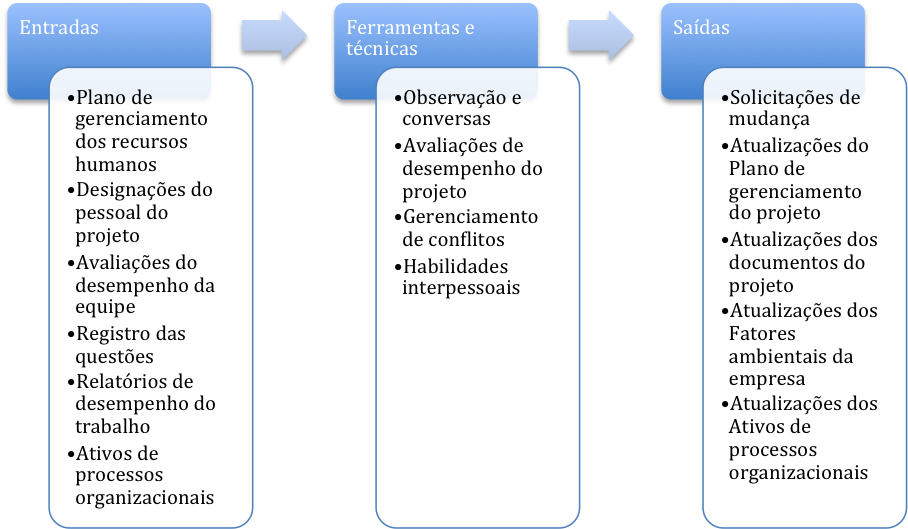
\includegraphics[scale=0.5]{Figuras/rh_efts_gerenciar.png}
	\caption{Gerenciar a equipe do projeto: entradas, ferramentas, técnicas e saídas}
	\label{fig:rh:ger:efts}
\end{figure}

\section{Entradas}

\begin{description}

	\item[Plano de gerenciamento dos recursos humanos:] inclui os papéis e responsabilidades, organização do projeto, plano de gerenciamento do pessoal, etc.
	
	\item[Designações do pessoal do projeto:] inclui a lista dos membros da equipe.
	
	\item[Avaliações do desempenho da equipe:] através da avaliação contínua do desempenho da equipe, ações podem ser tomadas para resolver problemas, modificar a comunicação, resolver conflitos e melhorar a interação da equipe.
	
	\item[Registro das questões:] usada para documentar e monitorar quem é responsável pela resolução de problemas específicos em uma data limite.
	
	\item[Relatórios de desempenho do trabalho:] auxilia na determinação de futuras necessidades de pessoal, reconhecimentos e recompensas e atualizações no plano de gerenciamento de pessoal.
	
	\item[Ativos de processos organizacionais:] certificados de apreciação, jornais internos, sites, estruturas de bônus, etc.
	
\end{description}

\section{Ferramentas e técnicas}

\begin{description}

	\item[Observação e conversas:] são usadas para manter contato com o trabalho e atitudes dos membros da equipe.
	
	\item[Avaliações de desempenho do projeto:] tem como objetivo clarificar os papéis e responsabilidades, fornecer feedback construtivo, descobrir problemas desconhecidos ou não resolvidos, desenvolver planos de treinamento e estabelecer objetivos específicos para períodos futuros.
	
	\item[Gerenciamento de conflitos:] resulta em uma maior produtividade e relacionamentos de trabalho positivos.
	
	\item[Habilidades interpessoais:] incluem principalmente liderança, influência e tomada de decisão efetiva.
		
\end{description}

\section{Saídas}

\begin{description}

	\item[Solicitações de mudança:] mudanças na equipe podem impactar no projeto e alterar o cronograma ou orçamento.
	
	\item[Atualizações do Plano de gerenciamento do projeto:] principalmente no plano de gerenciamento de recursos humanos.
	
	\item[Atualizações dos documentos do projeto:] registro de questões, descrição de papéis, designação de pessoal, etc.
	
	\item[Atualizações dos Fatores ambientais da empresa:] entrada para avaliação de desempenho organizacional, competências de pessoal, etc.
	
	\item[Atualizações dos Ativos de processos organizacionais:] informações históricas, lições aprendidas, modelos, processos padronizados, etc.
	
	
\end{description}
\chapter{Objetivos e características}

O gerenciamento das comunicações do projeto inclui os processos necessários para assegurar que as informações do projeto sejam geradas, coletadas, distribuídas, armazenadas, recuperadas e organizadas de maneira oportuna e apropriada.

Os processos que fazem parte do gerenciamento das comunicações, representados na Figura \ref{fig:proc:ger:comunic}, podem ser resumidos em:

\begin{description}
	
	\item[\textbf{Planejar o gerenciamento das comunicações}]: desenvolver uma aproximação apropriada e um plano para as comunicações do projeto baseado nas necessidades e requisitos de informações das partes interessadas e nos ativos organizacionais disponíveis.
	
	\item[\textbf{Gerenciar as comunicações}]: criar, coletar, distribuir, armazenar, recuperar e disponibilizar as informações do projeto de acordo com o plano de gerenciamento das comunicações.
	
	\item[\textbf{Controlar as comunicações}]: monitorar e controlar as comunicações durante todo o ciclo de vida do projeto para garantir que as necessidades de informações das partes interessadas do projeto sejam satisfeitas.

\end{description}

\begin{figure}[!h]
	\centering
	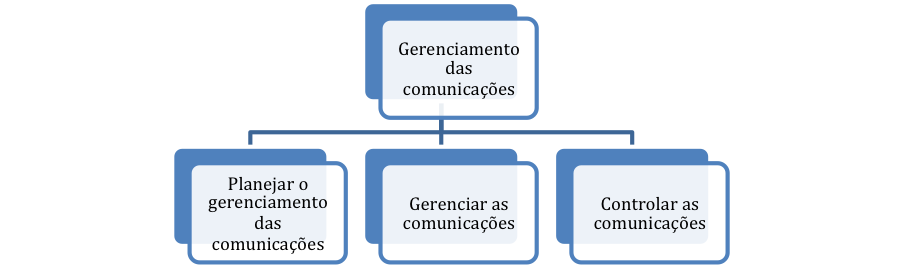
\includegraphics[scale=0.75]{Figuras/gerenciamento_comunicacoes.png}
	\caption{Processos do Gerenciamento das comunicações}
	\label{fig:proc:ger:comunic}
\end{figure}

\chapter{Planejar gerenciamento das comunicações}

O plano de gerenciamento das comunicações é o processo de desenvolver uma aproximação apropriada e um plano para as comunicações do projeto baseado nas necessidades e requisitos de informações das partes interessadas e nos ativos organizacionais disponíveis.

O processo de planejar o gerenciamento das comunicações está representado na Figura \ref{fig:comunic:plan:efts} e será descrito a seguir.

\begin{figure}[!h]
	\centering
	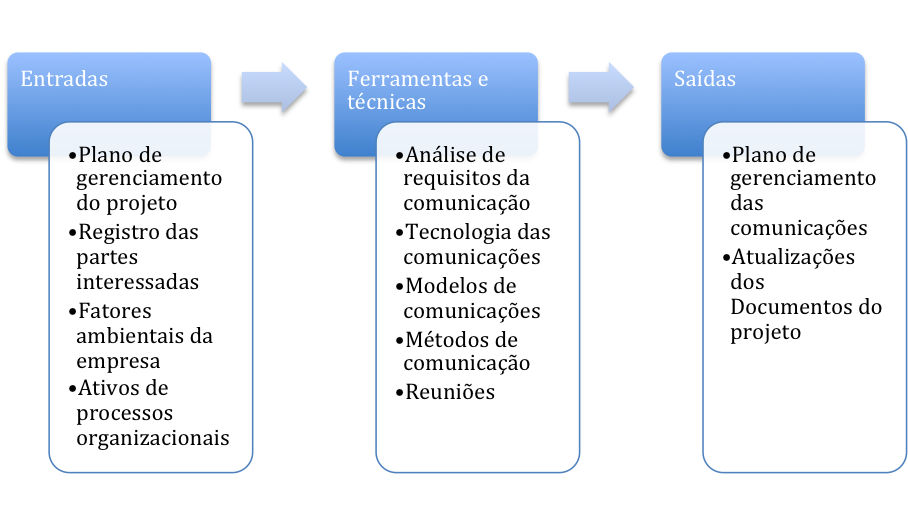
\includegraphics[scale=0.5]{Figuras/comunicacoes_efts_planejar.png}
	\caption{Planejar o gerenciamento das comunicações: entradas, ferramentas, técnicas e saídas}
	\label{fig:comunic:plan:efts}
\end{figure}

\section{Entradas}

\begin{description}
	
	\item[Plano de gerenciamento do projeto:] contém informações importantes para se executar, monitorar, controlar e encerrar o projeto.

	\item[Registro das partes interessadas:] contém necessidades e requisitos das partes interessadas.

	\item[Fatores ambientais da empresa:] intimamente ligado às comunicações, visto que a estrutura da organização terá um grande efeito nos requisitos das comunicações do projeto.

	\item[Ativos de processos organizacionais:] principalmente informações históricas e lições aprendidas, para avaliar as decisões tomadas sobre as comunicações e seus resultados.

\end{description}

\section{Ferramentas e técnicas}

\begin{description}

	\item[Análise de requisitos da comunicação:] determina a informação que as partes interessadas necessitam. Os requisitos são definidos pela combinação do tipo e formato da informação necessária através da análise do valor dessa informação.
	
	\item[Tecnologia das comunicações:] podem variar de acordo com a urgência da necessidade da informação, disponibilidade da tecnologia, facilidade de utilização, ambiente do projeto e sensibilidade e confiabilidade da informação.
	
	\item[Modelos de comunicações:] basicamente consiste no transmissor, receptor e meio. O transmissor é responsável pela tramissão da mensagem, pela garantia que a informação comunicada é clara e completa e pela confirmação que a comunicação foi corretamente entendida. O receptor é responsável por garantir que a informação foi recebida em sua totalidade, entendida corretamente e reconhecida ou respondida apropriadamente.
	
	\item[Métodos de comunicação:] de modo geral, são classifcadas em:
	
		\begin{description}
			
			\item[Comunicação interativa:] entre duas ou mais partes que estão realizando uma troca de informações multidirecional. É a forma mais eficiente de garantir um entendimento comum por todos os participantes sobre determinados tópicos. Inclui reuniões, telefonemas, videoconferências, etc.
			
			\item[Comunicação ativa (push):] encaminhada para destinatários específicos que precisam saber das informações. Garante que as informações sejam distribuídas mas não verifica se chegaram ou foram compreendidas pelo público-alvo. A comunicação ativa inclui cartas, memorandos, relatórios, emails, faxes, correio de voz, comunicados de imprensa, etc.
			
			\item[Comunicação passiva (pull):] usada para volumes muito grandes de informações ou para um público muito grande, requer que os destinatários acessem o conteúdo da comunicação a seu próprio critério. Esses métodos incluem sites de intranet, e-learning, repositórios de conhecimentos, etc.

		\end{description}	
		
	\item[Reuniões:] o planejamento do gerenciamento das comunicações requer discussões e diálogos com a equipe do projeto para determinar a forma mais apropriada de atualizar e comunicar as informações do projeto. Geralmente as reuniões facilitam essas discussões e diálogos.
	
\end{description}

\section{Saídas}

\begin{description}
	
	\item[Plano de gerenciamento das comunicações:] componente do \planproj que descreve como as comunicações do projeto serão planejadas, estruturadas, monitoradas e controladas.
	
	\item[Atualizações dos Documentos do projeto:] cronograma, registro de partes interessadas, etc.
	
\end{description}

\chapter{Gerenciar as comunicações}

Processo de criar, coletar, distribuir, armazenar, recuperar e disponibilizar as informações do projeto de acordo com o plano de gerenciamento das comunicações.

O processo de gerenciar as comunicações está representado na Figura \ref{fig:comunic:ger:efts} e será descrito a seguir.

\begin{figure}[!h]
	\centering
	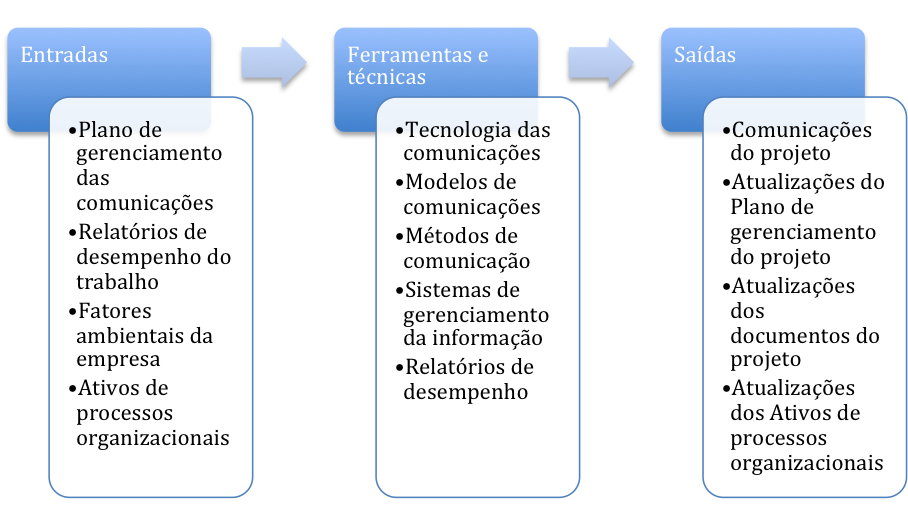
\includegraphics[scale=0.5]{Figuras/comunicacoes_efts_gerenciar.png}
	\caption{Gerenciar as comunicações: entradas, ferramentas, técnicas e saídas}
	\label{fig:comunic:ger:efts}
\end{figure}

\section{Entradas}

\begin{description}

	\item[Plano de gerenciamento das comunicações:] descreve como as comunicações do projeto serão planejadas, estruturadas, monitoradas e controladas.
	
	\item[Relatórios de desempenho do trabalho:] coleção de informações de performance e status do projeto que podem ser usadas para facilitar a discussão e criação das comunicações.
	
	\item[Fatores ambientais da empresa:] cultura e estrutura organizacional, padrões e regulamentações governamentais ou da indústria, sistemas de informação de gerência de projeto, etc.
	
	\item[Ativos de processos organizacionais:] políticas, procedimentos, processos e guias de gerenciamento de comunicações, modelos e informações históricas e lições aprendidas.

	
\end{description}

\section{Ferramentas e técnicas}

\begin{description}
	
	\item[Tecnologia das comunicações:] o foco é assegurar que a escolha seja apropriada para a informação que está sendo comunicada.
	
	\item[Modelos de comunicações:] o foco é assegurar que a escolha seja apropriada para o projeto e que barreiras (ruídos) sejam identificados e gerenciados.
	
	\item[Métodos de comunicação:] o foco é assegurar que a informação que foi criada e distribuída tenha sido recebida e compreendida para permitir resposta e feedback.
	
	\item[Sistemas de gerenciamento da informação:] ferramentas para gerenciar e distribuir informações do projeto.
	
	\item[Relatórios de desempenho:] ato de coletar e distribuir informações de desempenho, incluindo relatórios de status, medidads de progresso e previsões.
	
	
\end{description}

\section{Saídas}

\begin{description}
	
	\item[Comunicações do projeto:] relatórios de desempenho, status de entregas, progresso do cronograma, custos incorridos, etc.
	
	\item[Atualizações do Plano de gerenciamento do projeto:] o desempenho do projeto pode requerer alterações nas linhas de base do projeto.
	
	\item[Atualizações dos documentos do projeto:] o desempenho do projeto pode requerer alterações nos documentos do projeto.
	
	\item[Atualizações dos Ativos de processos organizacionais:] notificações de partes interessadas, relatórios do projeto, apresentações do projeto, registros do projeto, feedback das partes interessadas, lições aprendidas, etc.


\end{description}

\chapter{Controlar as comunicações}

Processo de monitorar e controlar as comunicações durante todo o ciclo de vida do projeto para garantir que as necessidades de informações das partes interessadas do projeto sejam satisfeitas.

O processo de controlar as comunicações está representado na Figura \ref{fig:comunic:controlar:efts} e será descrito a seguir.

\begin{figure}[!h]
	\centering
	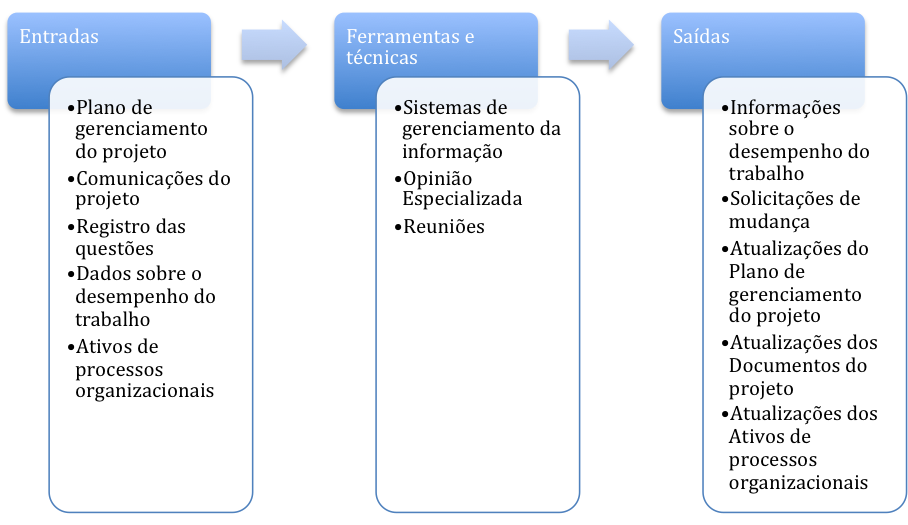
\includegraphics[scale=0.5]{Figuras/comunicacoes_efts_controlar.png}
	\caption{Controlar as comunicações: entradas, ferramentas, técnicas e saídas}
	\label{fig:comunic:controlar:efts}
\end{figure}

\section{Entradas}

\begin{description}

	\item[Plano de gerenciamento do projeto:] fornece os requisitos de comunicação das partes interessadas, razões para distruição das informações, tempo e frequência da distribuição das informações necessárias, responsáveis pelas comunicações das informações e receptores das informações.
	
	\item[Comunicações do projeto:] status das entregas, progresso do cronograma, custos incorridos, etc.
	
	\item[Registro das questões:] utilizado para documentar e monitorar a solução das questões.
	
	\item[Dados sobre o desempenho do trabalho:] detalhes sobre quais comunicações foram realmente distribuídas, feedbacks, pesquisas sobre efetividade das comunicações, etc.
	
	\item[Ativos de processos organizacionais:] modelos de relatórios, políticas, padrões e procedimentos que definem as comunicações, tecnologias disponíveis para comunicação, meios de comunicação permitidos, políticas de retenção de registros, requisitos de segurança, etc.
	
	
\end{description}

\section{Ferramentas e técnicas}

\begin{description}
	
	\item[Sistemas de gerenciamento da informação:] oferecem um conjunto de ferramentas padrão para o gerente de projetos capturar, armazenar e distribuir informações para as partes interessadas sobre os custos, cronograma e desempenho do projeto.
	
	\item[Opinião Especializada:] pode ser aplicada para detalhes técnicos e/ou gerenciais relativos às comunicações.
	
	\item[Reuniões:] facilitadoras de discussões e diálogos com a equipe de projeto que precisam determinar a forma mais apropriada de atualizar e comunicar o desempenho do projeto e responder às requisições de informações das partes interessadas.
	

\end{description}

\section{Saídas}

\begin{description}
	
	\item[Informações sobre o desempenho do trabalho:] organiza e sintetiza os dados de performance recolhidos.
	
	\item[Solicitações de mudança:] o processo de controle das comunicações geralmente resulta na necessidade de ajustes, ações e intervenções que, consequentemente, geram solicitações de mudanças.
	
	\item[Atualizações do Plano de gerenciamento do projeto:] planos de gerenciamento das partes interessadas e de recursos humanos, entre outros.
	
	\item[Atualizações dos Documentos do projeto:] previsões, relatórios de desempenho de trabalho, registro de questões, etc.
	
	\item[Atualizações dos Ativos de processos organizacionais:] formato de relatórios, documentação das lições aprendidas, etc.
	
\end{description}
% !TEX root = Apostila GP.tex

\capitulo{Riscos}

\secao{Objetivos e características}

O gerenciamento dos riscos do projeto inclui os processos necessários para aumentar a probabilidade e impacto de eventos positivos e diminuir a probabilidade de eventos negativos no projeto.

Os processos que fazem parte do gerenciamento dos riscos, representados na Figura \ref{fig:proc:ger:riscos}, podem ser resumidos em:

\begin{description}
	
	\item[Planejar o gerenciamento dos riscos:] definir como conduzir as atividades de gerenciamento de riscos para o projeto.

	\item[Identificar os riscos:] determinar quais riscos podem afetar o projeto e documentar suas características.

	\item[Realizar a análise qualitativa dos riscos:]  avaliar a exposição ao risco para priorizar os riscos que serão objeto de análise ou ação adicional.

	\item[Realizar a análise quantitativa dos riscos:] efetuar a análise numérica do efeito dos riscos identificados nos objetivos gerais do projeto.

	\item[Planejar as respostas aos riscos:] desenvolver opções e ações para aumentar as oportunidades e reduzir as ameaças aos objetivos do projeto.

	\item[Controlar os riscos:] monitorar e controlar os riscos durante o ciclo de vida do projeto.	

\end{description}

\begin{figure}[!h]
	\centering
	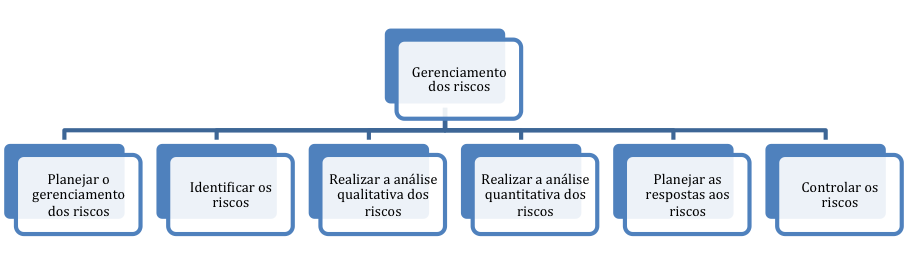
\includegraphics[scale=0.75]{Figuras/gerenciamento_riscos.png}
	\caption{Processos do Gerenciamento dos riscos}
	\label{fig:proc:ger:riscos}
\end{figure}

\secao{Planejar gerenciamento dos riscos}

O plano de gerenciamento dos riscos é o processo de como conduzir as atividades de gerenciamento dos riscos para um projeto.

O processo de planejar o gerenciamento dos riscos está representado na Figura \ref{fig:riscos:plan:efts} e será descrito a seguir.

\begin{figure}[!h]
	\centering
	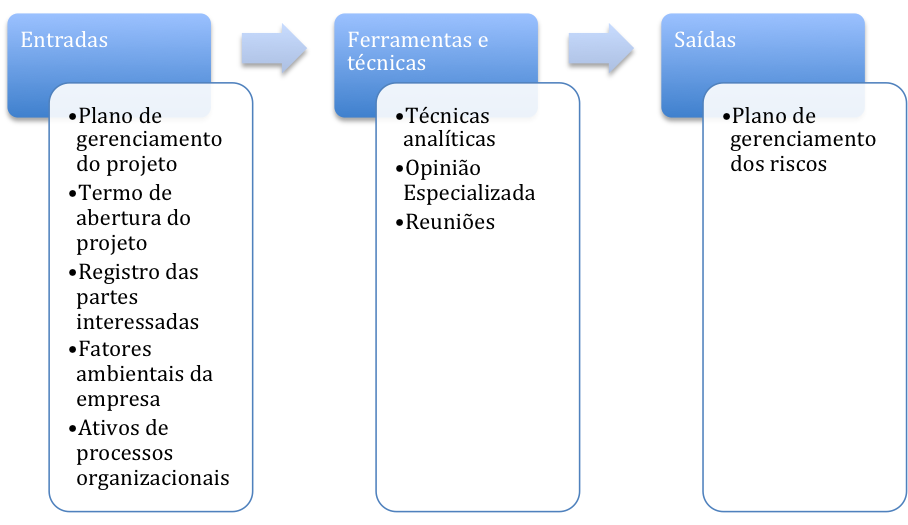
\includegraphics[scale=0.5]{Figuras/riscos_efts_planejar.png}
	\caption{Planejar o gerenciamento dos riscos: entradas, ferramentas, técnicas e saídas}
	\label{fig:riscos:plan:efts}
\end{figure}

\section{Entradas}

\begin{description}
	
	\item[Plano de gerenciamento do projeto:] todos os planos de gerenciamento subsidiários e linhas de base devem ser levados em consideração a fim de fazer com que o plano de gerenciamento de riscos esteja consistente com eles.
	
	\item[Termo de abertura do projeto:] contém os riscos em alto nível, descrições do projeto, requisitos de alto nível, etc.
	
	\item[Registro das partes interessadas:] oferece uma visão geral dos papéis das partes interessadas.
	
	\item[Fatores ambientais da empresa:] inclui atitudes, limites e tolerâncias aos riscos que caracterizam a resistência ao risco da organização.
	
	\item[Ativos de processos organizacionais:] categorias de riscos, definições de conceitos e termos, formatos de declaração de riscos, modelos, papéis e responsabilidades, nível de autoridade para tomada de decisões, lições aprendidas, etc.

\end{description}

\section{Ferramentas e técnicas}

\begin{description}

	\item[Técnicas analíticas:] utilizadas para entender e definir a visão geral do contexto do gerenciamento de riscos do projeto.
	
	\item[Opinião Especializada:] para garantir o estabelecimento compreensivo do plano de gerenciamento de riscos.
	
	\item[Reuniões:] para desenvolver o plano de gerenciamento de riscos.
	
\end{description}

\section{Saídas}

\begin{description}
	
	\item[Plano de gerenciamento dos riscos:] descreve como as atividade de gerenciamento de riscos serão estruturadas e realizadas.
	
\end{description}

\secao{Identificar os riscos}

Processo de determinar quais riscos podem afetar o projeto e documentar suas características.

O processo de identificar os riscos está representado na Figura \ref{fig:riscos:ident:efts} e será descrito a seguir.

\begin{figure}[!h]
	\centering
	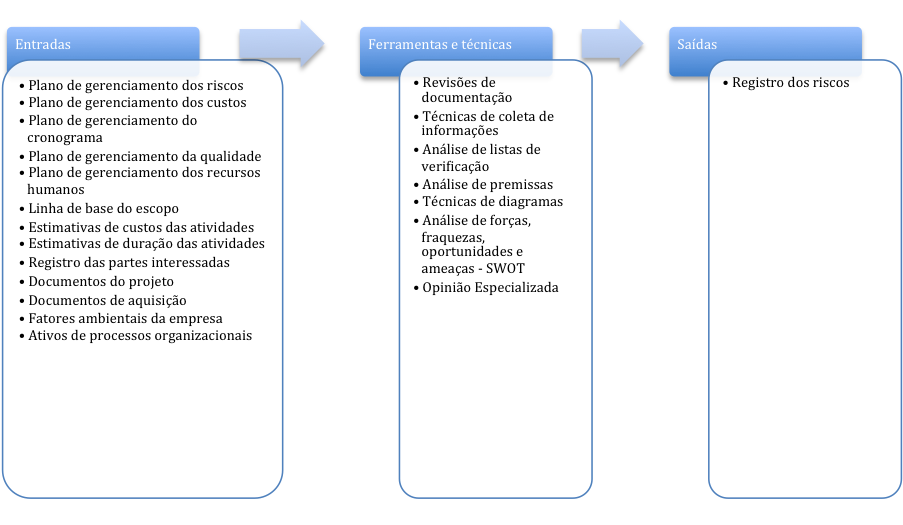
\includegraphics[scale=0.5]{Figuras/riscos_efts_identificar.png}
	\caption{Identificar os riscos: entradas, ferramentas, técnicas e saídas}
	\label{fig:riscos:ident:efts}
\end{figure}

\section{Entradas}

\begin{description}
	
	\item[Plano de gerenciamento dos riscos:] oferece elementos chave, tais como papéis e responsabilidades atribuídas, provisão no orçamento e cronograma para atividades de gerenciamento de riscos e categorias de riscos.
	
	\item[Plano de gerenciamento dos custos:] contém processos e controles que podem ser usados no auxílio da identificação de riscos.
	
	\item[Plano de gerenciamento do cronograma:] contém objetivos de cronograma que podem ser impactados pelos riscos.
	
	\item[Plano de gerenciamento da qualidade:] contém uma linha de base de medidas e métricas de qualidade para uso na identificação dos riscos.
	
	\item[Plano de gerenciamento dos recursos humanos:] contém papéis e responsabilidades, organogramas e planejamento de gerência de pessoal que são entradas chave para o processo de identificação dos riscos.
	
	\item[Linha de base do escopo:] contém as premissas que devem ser avaliadas como fontes potenciais de riscos.
	
	\item[Estimativas de custos das atividades:] a revisão das estimativas pode ser útil na identificação de riscos.
	
	\item[Estimativas de duração das atividades:] a revisão das estimativas pode ser útil na identificação de riscos.
	
	\item[Registro das partes interessadas:] as partes interessadas chave, especialmente o patrocinador e cliente, devem ser entrevistados ou participar na identificação dos riscos.
	
	\item[Documentos do projeto:] termo de abertura, cronograma, registro de questões, checklists de qualidade e outras informações que sejam valiosas na identificação dos riscos.
	
	\item[Documentos de aquisição:] quando for necessária a aquisição de recursos de fora, esses documentos se tornam chave no processo de identificação dos riscos.
	
	\item[Fatores ambientais da empresa:] informações publicadas, bancos de dados comerciais, estudos acadêmicos, checklists publicados, benchmarking, estudos da indústria, atidude aos riscos, etc.
	
	\item[Ativos de processos organizacionais:] arquivos de projetos, controles de processos organizacionais e de projeto, formatos e modelos de declaração de riscos, lições aprendidas, etc.
	
\end{description}

\section{Ferramentas e técnicas}

\begin{description}
	
	\item[Revisões de documentação:] a qualidade dos planos e a consistência entre eles e os requisitos e premissas pode ser um indicador de riscos do projeto.
	
	\item[Técnicas de coleta de informações:] brainstorming, técnica de Delphi, entrevistas, análise de causa raíz, etc.
	
	\item[Análise de listas de verificação:] pode-se criar uma lista de verificação de riscos.
	
	\item[Análise de premissas:] explorar a validade das premissas.
	
	\item[Técnicas de diagramas:] diagramas de causa e efeito, diagramas de fluxo de processo ou de sistema, diagrama de influência, etc.
	
	\item[Análise de forças, fraquezas, oportunidades e ameaças - SWOT:] utiliza essa visão para aumentar o alcance dos riscos.
	
	\item[Opinião Especializada:] qualquer profissional ou empresa que tenha experiência relevante em projetos ou áreas de negócios similares.

\end{description}

\section{Saídas}

\begin{description}
	
	\item[Registro dos riscos:] lista de riscos identificados e lista de potenciais respostas.
	
\end{description}

\secao{Realizar a análise qualitativa dos riscos}

Processo de avaliar a exposição ao risco para priorizar os riscos que serão objeto de análise ou ação adicional.

O processo de realizar a análise qualitativa dos riscos está representado na Figura \ref{fig:riscos:analise:qual:efts} e será descrito a seguir.

\begin{figure}[!h]
	\centering
	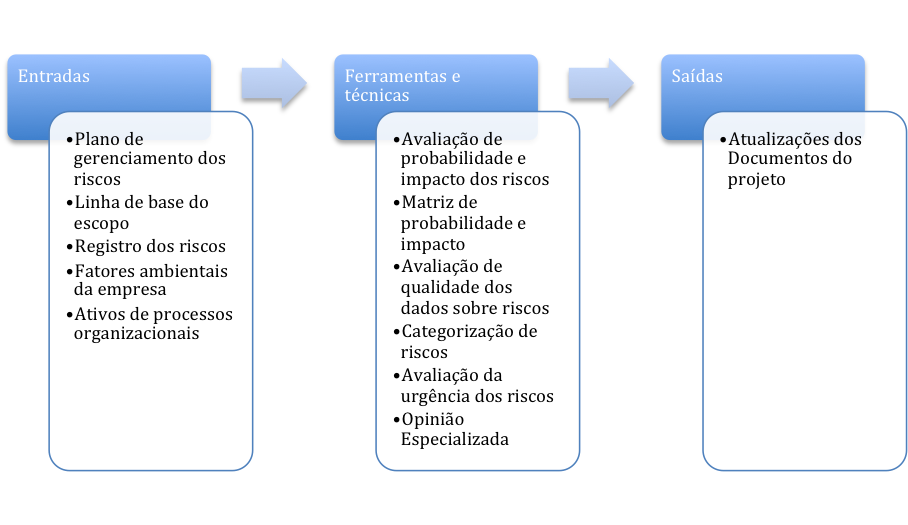
\includegraphics[scale=0.5]{Figuras/riscos_efts_analise_qual.png}
	\caption{Realizar a análise qualitativa dos riscos: entradas, ferramentas, técnicas e saídas}
	\label{fig:riscos:analise:qual:efts}
\end{figure}

\section{Entradas}

\begin{description}
	\item[Plano de gerenciamento dos riscos:] contém diversos elementos chave para análise dos riscos.
	
	\item[Linha de base do escopo:] auxilia na análise da complexidade do projeto.
	
	\item[Registro dos riscos:] contém informações para avaliar e priorizar os riscos.
	
	\item[Fatores ambientais da empresa:] estudos de especialista sobre riscos de projetos similares, bancos de dados de riscos, etc.
	
	\item[Ativos de processos organizacionais:] informações de projetos finalizados similares.

\end{description}

\section{Ferramentas e técnicas}

\begin{description}
		\item[Avaliação de probabilidade e impacto dos riscos:] investiga a probabilidade de cada risco específico ocorrer.
		
		\item[Matriz de probabilidade e impacto:] avaliação da importância e prioridade de atenção de cada risco é tipicamente conduzida usando uma tabela ou matriz de probabilidade e impacto.
		
		\item[Avaliação de qualidade dos dados sobre riscos:] avaliação do grau de utilidade dos dados sobre riscos.
		
		\item[Categorização de riscos:] os riscos podem ser categorizados pela fonte, área do projeto afetada ou outras categorias úteis.
		
		\item[Avaliação da urgência dos riscos:] riscos com respostas de curto prazo podem ser considerados mais urgentes.
		
		\item[Opinião Especializada:] auxiliam na avaliação da probabilidade  e impacto de cada risco.
		
\end{description}

\section{Saídas}

\begin{description}
	
	\item[Atualizações dos Documentos do projeto:] registro de riscos, registro de premissas, etc.
	
\end{description}

\secao{Realizar a análise quantitativa dos riscos}

Processo de efetuar a análise numérica do efeito dos riscos identificados nos objetivos gerais do projeto.

O processo de realizar a análise quantitativa dos riscos está representado na Figura \ref{fig:riscos:analise:quant:efts} e será descrito a seguir.

\begin{figure}[!h]
	\centering
	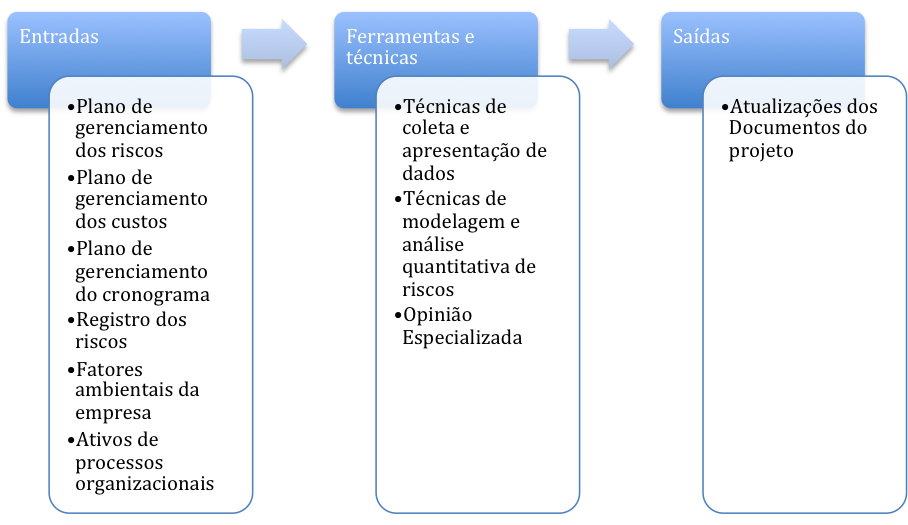
\includegraphics[scale=0.5]{Figuras/riscos_efts_analise_quant.png}
	\caption{Realizar a análise quantitativa dos riscos: entradas, ferramentas, técnicas e saídas}
	\label{fig:riscos:analise:quant:efts}
\end{figure}

\section{Entradas}

\begin{description}
	
	\item[Plano de gerenciamento dos riscos:] contém os guias, métodos e ferramentas utilizadas na análise quantitativa.
	
	\item[Plano de gerenciamento dos custos:] contém os guias para estabelecer e gerenciar as reservas de risco.
	
	\item[Plano de gerenciamento do cronograma:] contém os guias para estabelecer e gerenciar as reservas de risco.
	
	\item[Registro dos riscos:] ponto de referência para realizar a análise.
	
	\item[Fatores ambientais da empresa:] estudos realizados por especialistas sobre riscos similares, bancos de dados de riscos, etc.
	
	\item[Ativos de processos organizacionais:] informações sobre projetos finalizados similares.
	
\end{description}

\section{Ferramentas e técnicas}

\begin{description}

	\item[Técnicas de coleta e apresentação de dados:] entrevistas, distribuição de probabilidades, etc.
	
	\item[Técnicas de modelagem e análise quantitativa de riscos:] análise de sensibilidade, análise de valor monetário esperado, modelagem e simulação, etc.
	
	\item[Opinião Especializada:] auxilia na identificação de pontenciais custos e impactos no cronograma, na avaliação de probabilidades, etc.
	
\end{description}

\section{Saídas}

\begin{description}
	
	\item[Atualizações dos Documentos do projeto:] análise probabilística do projeto, probabilidade de atingir os objetivos de custo e tempo, lista priorizada de riscos quantificados, tendências nos resultados de análise quantitativa dos riscos, etc.	
	
\end{description}


\secao{Planejar as respostas aos riscos}

Processo de desenvolver opções e ações para aumentar as oportunidades e reduzir as ameaças aos objetivos do projeto.

O processo de planejar as respostas aos riscos está representado na Figura \ref{fig:riscos:resp:efts} e será descrito a seguir.

\begin{figure}[!h]
	\centering
	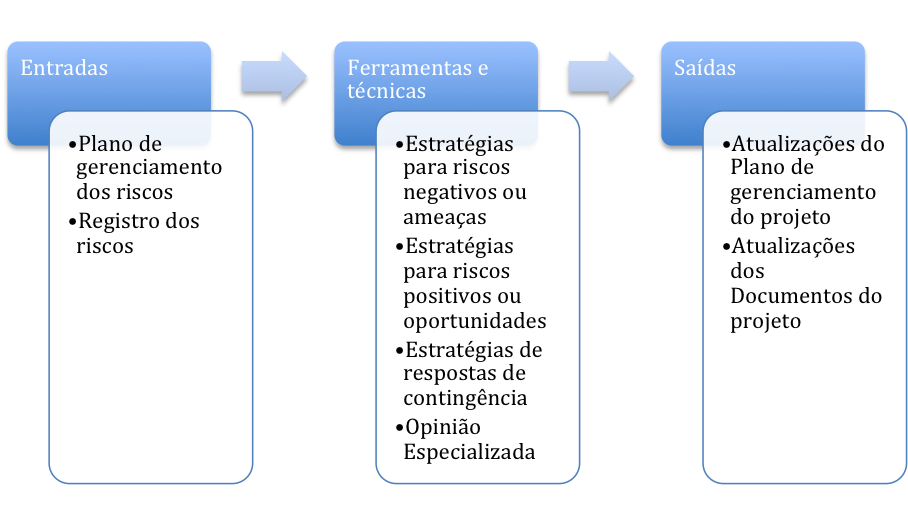
\includegraphics[scale=0.5]{Figuras/riscos_efts_resp.png}
	\caption{Planejar as respostas aos riscos: entradas, ferramentas, técnicas e saídas}
	\label{fig:riscos:resp:efts}
\end{figure}

\section{Entradas}

\begin{description}
	
	\item[Plano de gerenciamento dos riscos:] inclui papéis e responsabilidades, definições de análise de riscos, tempo para revisões, limites dos riscos, etc.
	
	\item[Registro dos riscos:] identifica os riscos, as causas raíz, lista de pontenciais respostas, etc.
	
\end{description}

\section{Ferramentas e técnicas}

\begin{description}
	
	\item[Estratégias para riscos negativos ou ameaças:] evitar, transferir, mitigar, aceitar.
	
	\item[Estratégias para riscos positivos ou oportunidades:] explorar, aumentar, compartilhar, aceitar.
	
	\item[Estratégias de respostas de contingência:] plano para respostas que serão executadas somente quando (e se) determinados eventos ocorrerem.
	
	\item[Opinião Especializada:] auxiliam com conhecimento sobre ações pertinentes às ações que devem ser tomadas para um determinado risco.
	
\end{description}

\section{Saídas}

\begin{description}
	
	\item[Atualizações do Plano de gerenciamento do projeto:] planos de gerenciamento do cronograma, custos, qualidade, aquisições e RH, além das linhas de base do escopo, cronograma e custo.
	
	\item[Atualizações dos Documentos do projeto:] diversos documentos auxiliares podem ser afetados pelas respostas aos riscos.	
	
\end{description}


\secao{Controlar os riscos}

Processo de monitorar e controlar os riscos durante o ciclo de vida do projeto.

O processo de controlar os riscos está representado na Figura \ref{fig:riscos:controlar:efts} e será descrito a seguir.

\begin{figure}[!h]
	\centering
	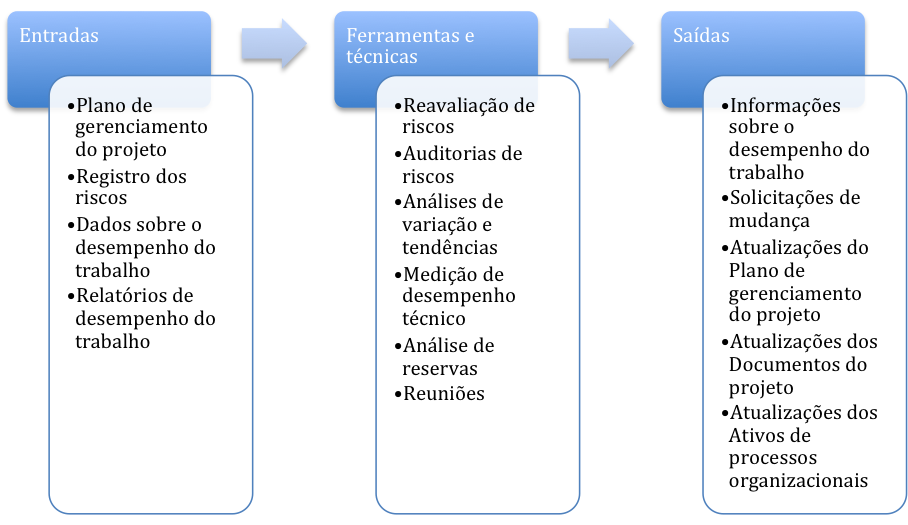
\includegraphics[scale=0.5]{Figuras/riscos_efts_controlar.png}
	\caption{controlar os riscos: entradas, ferramentas, técnicas e saídas}
	\label{fig:riscos:controlar:efts}
\end{figure}

\section{Entradas}

\begin{description}
	
	\item[Plano de gerenciamento do projeto:] contém guias para monitorar e controlar os riscos.
	
	\item[Registro dos riscos:] contém os riscos que devem ser monitorados e controlados.
	
	\item[Dados sobre o desempenho do trabalho:] status das entregas, progresso do cronograma, custos incorridos, etc.
	
	\item[Relatórios de desempenho do trabalho:] contém dados que podem impactar o controle de riscos relacionados com o desempenho.	
	
\end{description}

\section{Ferramentas e técnicas}

\begin{description}
	
	\item[Reavaliação de riscos:] o controle de riscos pode resultar na identificação de novos riscos.
	
	\item[Auditorias de riscos:] examina e documenta a efetividade das respostas aos riscos.
	
	\item[Análises de variação e tendências:] podem prever ponteciais desvios de custo e cronograma, indicadores de ponteciais riscos.
	
	\item[Medição de desempenho técnico:] podem prever o nível de sucesso para alcançar o escopo do projeto.
	
	\item[Análise de reservas:] compara a quantia da reserva de contingência remanescente com os riscos remanescentes para verificar se a reserva é suficiente.
	
	\item[Reuniões:] o gerenciamento de riscos deve constar da agenda de reuniões periódicas de desempenho.
	
\end{description}

\section{Saídas}

\begin{description}
	
	\item[Informações sobre o desempenho do trabalho:] oferece um mecanismo para comunicar e auxiliar o processo de tomada de decisão do projeto.
	
	\item[Solicitações de mudança:] ações corretivas e preventivas recomendadas.
	
	\item[Atualizações do Plano de gerenciamento do projeto:] planos de gerenciamento do cronograma, custos, qualidade, aquisições e RH, além das linhas de base do escopo, cronograma e custo
	
	\item[Atualizações dos Documentos do projeto:] saídas de avaliação de riscos, auditorias de riscos, revisões periódicas de riscos e saídas reais dos riscos e respostas.
	
	\item[Atualizações dos Ativos de processos organizacionais:] modelos do plano de gerenciamento de riscos, estrutura analítica de riscos, lições aprendidas, etc.
	
\end{description}
\chapter{Objetivos e características}

O gerenciamento das partes interessadas do projeto inclui os processos necessários para identificar as pessoas, grupos ou organizações que podem impactar ou serem impactadas pelo projeto, analisar as suas expectativas e impactos no projeto e desenvolver estratégias apropriadas para efetivamente engajar as partes interessadas nas decisões e execuções do projeto.

Os processos que fazem parte do gerenciamento das partes interessadas, representados na Figura \ref{fig:proc:ger:stakeholders}, podem ser resumidos em:

\begin{description}

	\item[Identificar as partes interessadas:] identificar as pessoas, grupos ou organizações que podem impactar ou serem impactadas por uma decisão, atividade ou resultado do projeto; analisar e documentar informações relavantes sobre seus interesses, envolvimentos, interdependências, influência e potencial impacto no sucesso do projeto.
	
	\item[Planejar o gerenciamento das partes interessadas:] desenvolver estratégias para efetivamente engajar as partes interessadas durante o ciclo de vida do projeto, baseado na análise de suas necessidades, interesses e potenciais impactos no sucesso do projeto.
	
	\item[Gerenciar o engajamento das partes interessadas:] comunicar e interagir com as partes interessadas para atender suas necessidades, solucionar as questões quando ocorrem e fomentar o engajamento nas atividades durante todo o ciclo de vida do projeto.
	
	\item[Controlar o engajamento das partes interessadas:] monitorar os relacionamentos entre as partes interessadas e ajustar as estratégias para engajar as partes interessadas eliminando resistências e aumentando o suporte ao projeto.

\end{description}

\begin{figure}[!h]
	\centering
	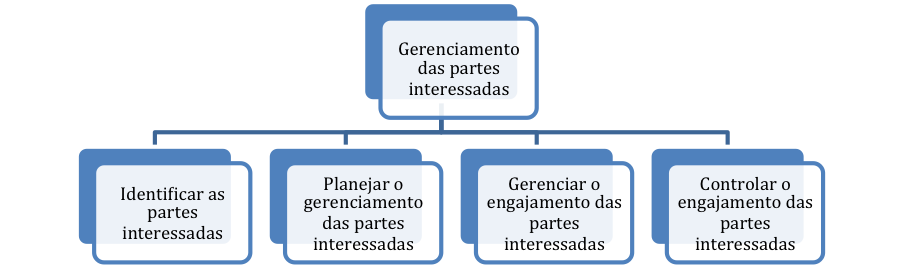
\includegraphics[scale=0.75]{Figuras/gerenciamento_stakeholders.png}
	\caption{Processos do Gerenciamento das partes interessadas}
	\label{fig:proc:ger:stakeholders}
\end{figure}

\chapter{Identificar as partes interessadas}

Processo de identificar as pessoas, grupos ou organizações que podem impactar ou serem impactadas por uma decisão, atividade ou resultado do projeto; analisar e documentar informações relavantes sobre seus interesses, envolvimentos, interdependências, influência e potencial impacto no sucesso do projeto.

O processo de identificar as partes interessadas está representado na Figura \ref{fig:sh:id:efts} e será descrito a seguir.

\begin{figure}[!h]
	\centering
	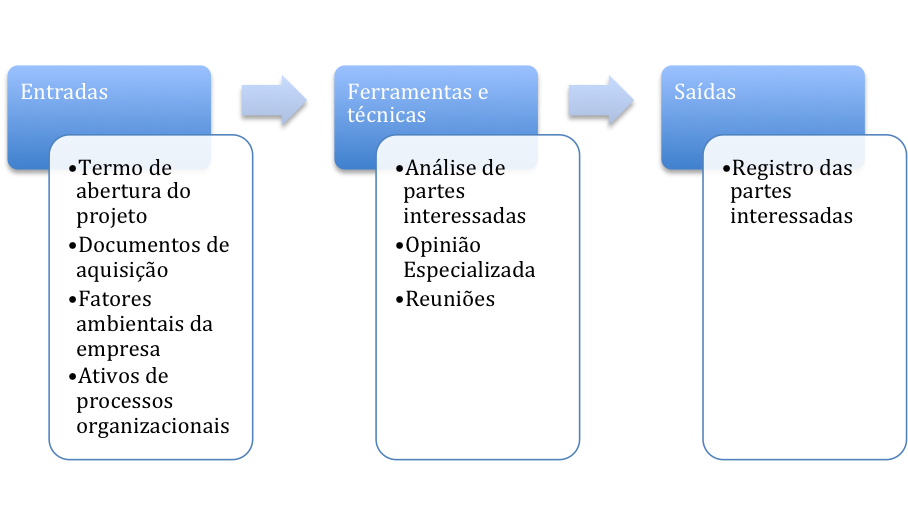
\includegraphics[scale=0.5]{Figuras/stakeholders_efts_identificar.png}
	\caption{Identificar as partes interessadas: entradas, ferramentas, técnicas e saídas}
	\label{fig:sh:id:efts}
\end{figure}

\section{Entradas}

\begin{description}

	\item[Termo de abertura do projeto:] fornece informações sobre partes internas e externas relacionadas com o projeto, tais como: patrocinador, clientes, equipe, grupos, departamentos e outras organizações.
	
	\item[Documentos de aquisição:] as partes dos contratos e os fornecedores são partes interessadas chaves do projeto.
	
	\item[Fatores ambientais da empresa:] cultura e estrutura organizacional, padrões governamentais e da indústria, práticas e hábitos globais ou regionais.
	
	\item[Ativos de processos organizacionais:]	modelos de registro de partes interessadas, lições aprendidas, registros de partes interessadas de projetos anteriores, etc.

\end{description}

\section{Ferramentas e técnicas}

\begin{description}
	
	\item[Análise de partes interessadas:] técnica de sistematicamente juntar e analisar quantitativamente e qualitativamente informações para determinar quais interesses devem ser levados em consideração durante o projeto.
	
	\item[Opinião Especializada:] auxilia na identificação e listagem das partes interessadas.
	
	\item[Reuniões:] podem auxiliar na análise de perfil das partes interessadas.

\end{description}

\section{Saídas}

\begin{description}

	\item[Registro das partes interessadas:] contém informações de identificação, avaliação e classificação das partes interessadas.
	
\end{description}

\chapter{Planejar o gerenciamento das partes interessadas}

Processo de desenvolver estratégias para efetivamente engajar as partes interessadas durante o ciclo de vida do projeto, baseado na análise de suas necessidades, interesses e potenciais impactos no sucesso do projeto.

O processo de planejar o gerenciamento das partes interessadas está representado na Figura \ref{fig:sh:ger:efts} e será descrito a seguir.

\begin{figure}[!h]
	\centering
	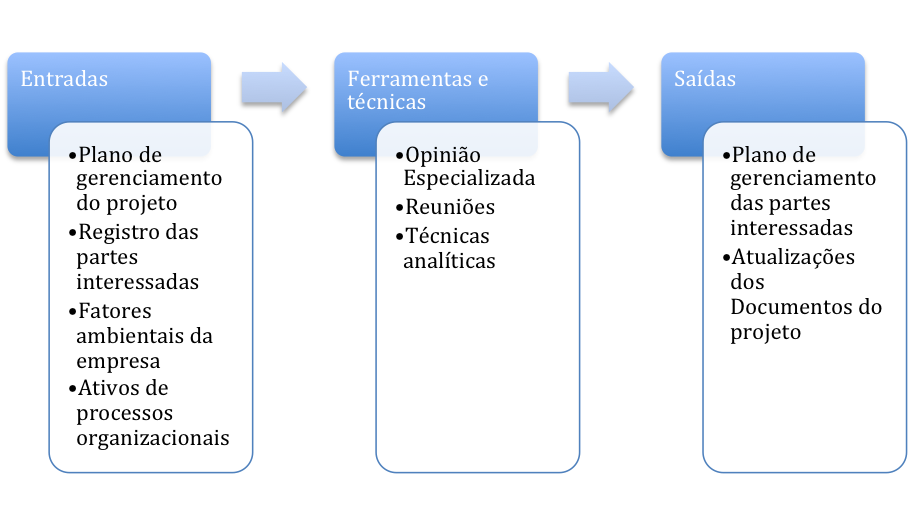
\includegraphics[scale=0.5]{Figuras/stakeholders_efts_gerenciar.png}
	\caption{Planejar o gerenciamento das partes interessadas: entradas, ferramentas, técnicas e saídas}
	\label{fig:sh:ger:efts}
\end{figure}

\section{Entradas}

\begin{description}
	
	\item[Plano de gerenciamento do projeto:] inclui o ciclo de vida selecionado para o projeto e os processos que serão aplicados em cada fase, descrição de como o trabalho será executado para alcançar os objetivos do projeto, descrição de como os requisitos de recursos humanos serão atendidos, descrição de como as mudanças serão controladas, necessidades e técnicas de comunicação entre as partes interessadas, etc.
	
	\item[Registro das partes interessadas:] fornece informações necessárias para planejar as formas de engajar as partes interessadas no projeto.
	
	\item[Fatores ambientais da empresa:] cultura, estrutura, clima e política organizacional, entre outros.
	
	\item[Ativos de processos organizacionais:] lições aprendidas, informações históricas, etc.
	
\end{description}

\section{Ferramentas e técnicas}

\begin{description}
	
	\item[Opinião Especializada:] auxilia na decisão do nível de engajamento necessário a cada estágio do projeto para cada parte interessada.
	
	\item[Reuniões:] utilizadas para determinar o nível de engajamento necessário de todas as partes interessadas.
	
	\item[Técnicas analíticas:] comparação do nível corrente de engajamento com o nível planejado.
		
\end{description}

\section{Saídas}

\begin{description}

	\item[Plano de gerenciamento das partes interessadas:] identifica as estratégias necessárias para efetivamente engajar as partes interessadas.
	
	\item[Atualizações dos Documentos do projeto:] cronograma, registro de partes interessadas, etc.
	
\end{description}

\chapter{Gerenciar o engajamento das partes interessadas}
Processo de comunicar e interagir com as partes interessadas para atender suas necessidades, solucionar as questões quando ocorrem e fomentar o engajamento nas atividades durante todo o ciclo de vida do projeto.

O processo de gerenciar o engajamento das partes interessadas do projeto está representado na Figura \ref{fig:sh:engaja:ger:efts} e será descrito a seguir.

\begin{figure}[!h]
	\centering
	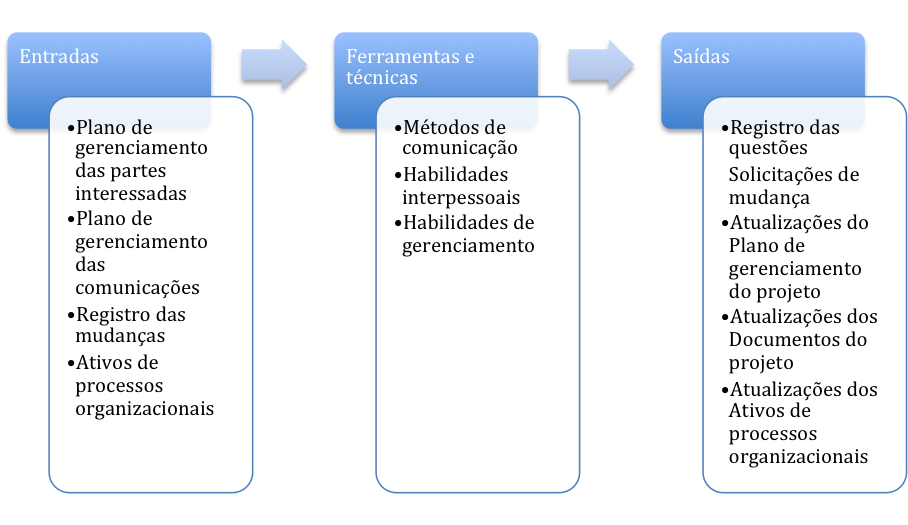
\includegraphics[scale=0.5]{Figuras/stakeholders_efts_ger_engaja.png}
	\caption{Gerenciar o engajamento das partes interessadas: entradas, ferramentas, técnicas e saídas}
	\label{fig:sh:engaja:ger:efts}
\end{figure}

\section{Entradas}

\begin{description}

	\item[Plano de gerenciamento das partes interessadas:] oferece orientações sobre como as várias partes interessadas podem ser melhor envolvidas no projeto.
	
	\item[Plano de gerenciamento das comunicações:] oferece orientações e informações sobre as expectativas das partes interessadas.
	
	\item[Registro das mudanças:] utilizado para documentar as mudanças que ocorrem durante o projeto.
	
	\item[Ativos de processos organizacionais:] requisitos de comunicação organizacional, procedimentos de gerência de questões, procedimentos de controle de mudanças, informações históricas, etc.
	

\end{description}

\section{Ferramentas e técnicas}

\begin{description}
	
	\item[Métodos de comunicação:] identificados para cada parte interessada.
	
	\item[Habilidades interpessoais:] construir confiança, resolver conflitos, escuta ativa, superar resistência à mudança, etc.
	
	\item[Habilidades de gerenciamento:] facilitar consenso em direção aos objetivos do projeto, influenciar pessoas a apoiar o projeto, negociar acordos para satisfazer necessidades do projeto, modificar comportamento organizacional para obter aceite dos resultados do projeto, etc.
	
\end{description}

\section{Saídas}

\begin{description}
	
	\item[Registro das questões:] gerenciar as partes interessadas pode resultar em questões que devem ser registradas.
	
	\item[Solicitações de mudança:] gerenciar as partes interessadas pode resultar em mudanças.
	
	\item[Atualizações do Plano de gerenciamento do projeto:] ocorrem quando requisitos novos ou modificados são identificados.
	
	\item[Atualizações dos Documentos do projeto:] registro de partes interessadas, entre outros.
	
	\item[Atualizações dos Ativos de processos organizacionais:] notificações das partes interessadas, relatórios, apresentações, registros, feedback das partes interessadas, lições aprendidas, etc.
	
\end{description}

\chapter{Controlar o engajamento das partes interessadas}

Processo de monitorar os relacionamentos entre as partes interessadas e ajustar as estratégias para engajar as partes interessadas eliminando resistências e aumentando o suporte ao projeto.

O processo de controlar o engajamento das partes interessadas está representado na Figura \ref{fig:rh:engaja:cont:efts} e será descrito a seguir.

\begin{figure}[!h]
	\centering
	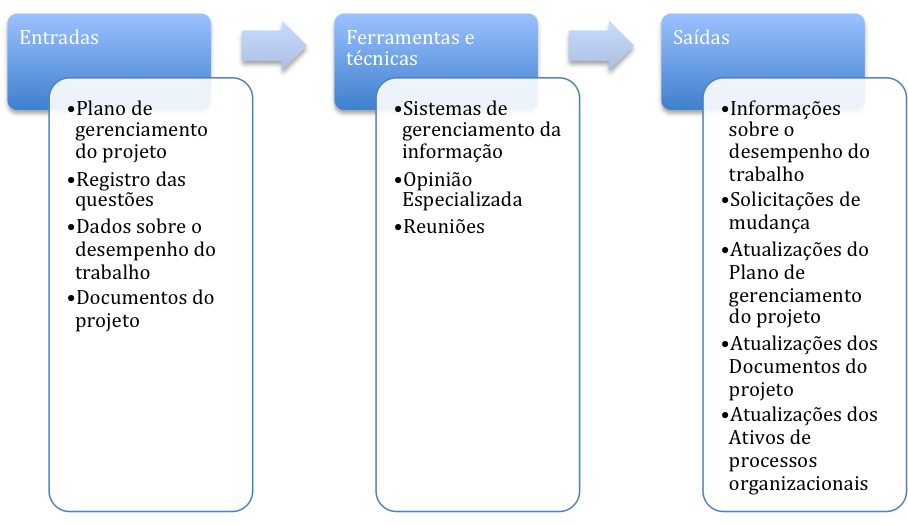
\includegraphics[scale=0.5]{Figuras/stakeholders_efts_cont_engaja.png}
	\caption{Controlar o engajamento das partes interessadas: entradas, ferramentas, técnicas e saídas}
	\label{fig:rh:engaja:cont:efts}
\end{figure}

\section{Entradas}

\begin{description}	

	\item[Plano de gerenciamento do projeto:] inclui o ciclo de vida selecionado para o projeto e os processos que serão aplicados em cada fase, descrição de como o trabalho será executado para alcançar os objetivos do projeto, descrição de como os requisitos de recursos humanos serão atendidos, descrição de como as mudanças serão controladas, necessidades e técnicas de comunicação entre as partes interessadas, etc.
	
	\item[Registro das questões:] atualizado conforme novas questões aparecem e as atuais são resolvidas.
	
	\item[Dados sobre o desempenho do trabalho:] observações e medições identificadas durante a execução das atividades do projeto.
	
	\item[Documentos do projeto:] cronograma, registro de partes interessadas, registro de questões, registro de mudanças, comunicações do projeto, etc.
	
\end{description}

\section{Ferramentas e técnicas}

\begin{description}

	\item[Sistemas de gerenciamento da informação:] capturam, armazenam e distribuem informações para as partes interessadas a respeito de custos, progresso do cronograma e desempenho do projeto.
	
	\item[Opinião Especializada:] garantir identificação e listagem de novas partes interessadas e reavaliação das atuais.
	
	\item[Reuniões:] utilizadas para troca e análise de informações sobre engajamento das partes interessadas.
			
\end{description}

\section{Saídas}

\begin{description}
	
	\item[Informações sobre o desempenho do trabalho:] status das entregas, status de implementação para solicitação de mudanças, etc.
	
	\item[Solicitações de mudança:] análise de desempenho e interação com as partes interessadas geralmente geram solicitações de mudanças.
	
	\item[Atualizações do Plano de gerenciamento do projeto:] plano de gerenciamento de mudanças, plano de gerenciamento de comunicações, plano de gerenciamento de custos, plano de gerenciamento de RH, plano de gerenciamento de qualidade, plano de gerenciamento de requisitos, plano de gerenciamento de riscos, plano de gerenciamento de cronograma, plano de gerenciamento de escopo, plano de gerenciamento de partes interessadas, etc.
	
	\item[Atualizações dos Documentos do projeto:] registro de partes interessadas, registro de questões, etc.
	
	\item[Atualizações dos Ativos de processos organizacionais:] notificações das partes interessadas, relatórios, apresentações, registros, feedback das partes interessadas, lições aprendidas, etc.
	
\end{description}
%% !TEX root = Apostila GP.tex

\chapter{Ferramentas de TI}

\section{Microsoft Project}

Um dos \sws mais conhecidos de gerenciamento de projetos, se destaca pela sua facilidade de utilização. Aqui apresentaremos algumas das principais funcionalidades da versão 2010.

\subsection{Primeiros passos}

Ao entrar pela primeira vez no \msp, você irá visualizar o modo padrão de exibição, chamado de diagrama de Gantt, pronto para receber dados de seu projeto, conforme as Figuras \ref{fig:msp:tela1} e \ref{fig:msp:tela2}.

\begin{figure}[!h]
\centering
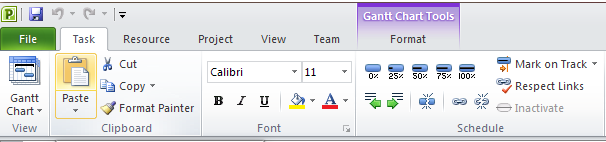
\includegraphics[scale=0.45]{Figuras/project_inicio1.png}
\caption{Guias de comandos e opções do \msp}
\label{fig:msp:tela1}
\end{figure}

\begin{figure}[!h]
\centering
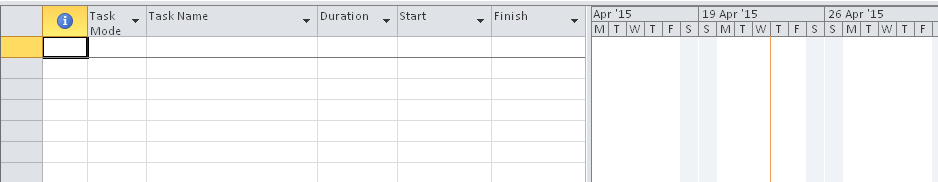
\includegraphics[scale=0.45]{Figuras/project_inicio2.png}
\caption{Tarefas e cronograma do \msp}
\label{fig:msp:tela2}
\end{figure}

Além do modo padrão de exibição, é possível escolher entre outros diversos modos e até mesmo criar o seu próprio modelo. Para isso, basta clicar no botão Gantt Chart (Figura \ref{fig:msp:tela3}) e selecionar um dos modos disponíveis.

\begin{figure}[!h]
\centering
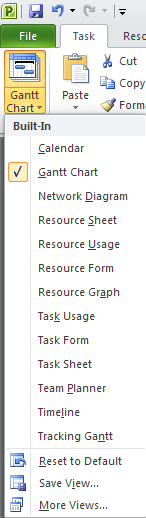
\includegraphics[scale=0.55]{Figuras/project_inicio3.png}
\caption{Botão para troca de modo de visualização}
\label{fig:msp:tela3}
\end{figure}


%\bibliographystyle{plain}
%\bibliographystyle{bibstyle/latex8}     
%\bibliographystyle{apalike-url}     


\bibliographystyle{Bibliografia/apalike-pt}     

%\bibliographystyle{lastchecked}     
            
\bibliography{Bibliografia/research}

\end{document}